\section{Related Work}

Many researchers have studied using smartphone sensors for continuous user authentication.
The benefit of continuous user authentication is that it happens unobtrusively, without requiring any action from users.
Continuous authentication could serve as a mitigation for theft: if the phone can detect rapidly enough that it is no longer being used by the rightful owner, it could lock itself to prevent the thief from accessing sensitive data on the phone. 


One approach is to use smartphone accelerometer data for gait recognition.
These systems often extract some features from the sensor data and then apply machine learning.
Derawi et~al.\ achieved an equal error rate of 20\%~\cite{derawi:gait}.
``Equal error rate'' is a measure of accuracy where the system is tuned so the false accept rate and false reject rates are equal, and then that error rate is reported.
Primo et~al.\ show that accelerometer-based gait authentication is somewhat dependent on the position in which the phone is held, which is a challenge for deploying gait authentication outside of a laboratory environment~\cite{primo:context}. 
They showed how to infer the position of the phone (in the person's hand vs in their pocket) with 85\% accuracy, and they showed how to use this information to increase the accuracy of user authentication to 70--80\%.
They do not report performance as equal error rate.
Juefei-Xu et~al.\ show that the pace at which people walk also affects the sensor readings, and it is possible to improve accuracy by first identifying the pace at which the user is walking, then using a model tailored towards that pace~\cite{xu:pace}.
Their system achieved an equal error rate of 4--8\% (depending on the pace); or a false reject rate of 0.5--5\% at a false accept rate of 0.1\%.
Kwapisz et~al.\ generalized gait authentication to cover not just walking but also jogging and ascending and descending stairs~\cite{kwapisz:biometrics} and
achieved false reject rates of 10--15\% at a false accept rate of about 5\%.

It is not clear whether gait recognition is sufficient on its own for deployable user authentication.
One limitation is that it can only attempt to authenticate the user while the user is walking; when the user is still, it cannot infer user identity.
Another limitation is that the error rate is still fairly high: if the classifier is run continuously, once per second, even a false reject rate as low as 0.5\% will cause hundreds or thousands of false rejections per week.
Thus, gait recognition might need to be combined with other methods to yield a deployable defense against theft.

We learned from the methods they used to process sensor data and extract features.
The accelerometer sensor provides raw data in the form of $X,Y,Z$ accelerations; it is useful to also compute the magnitude $M=\sqrt{X^2+Y^2+Z^2}$ of the acceleration, as that is independent of the direction of the acceleration.
Prior papers use several methods for cleaning the raw accelerometer data, including interpolation and re-sampling to deal with irregularly sampled data and a weighted moving average filter to mitigate sensor noise.
These schemes typically divide the resulting time series into windows, each window containing about a second of sensor data.
For instance, Primo et~al.\ use overlapping windows, with each window containing 100 samples and having an overlap of 50 samples with the next window; Derawi et~al.\ and Juefei-Xu et~al.\ use non-overlapping windows about 1 second in width.
Derawi et~al.\ and Juefei-Xu et~al.\ use the sensor readings as the features, while Primo et~al.\ and Kwapisz et~al.\ compute hand-crafted features from the readings, where each feature records a summary statistic on the sensor readings in the window (e.g., mean, minimum, maximum, standard deviation, number of zero crossings, etc.).

Feng et~al.\ investigated using the unique way the user picks up their phone as a biometric for user authentication~\cite{feng:pickup}. 
They achieve equal error rate of 6--7\%.
They use the smartphone accelerometer, gyroscope, and magnetometer; in our work, we avoid the gyroscope sensor, as its power consumption is significantly higher than the accelerometer.

Mare et~al.\ developed a continuous authentication system where the user wears a smartwatch or bracelet, which is used to authenticate the user to their computer~\cite{mare:zebra}. 
Their continuous authentication scheme works well and could plausibly be used to authenticate to a smartphone, but it requires users to wear a bracelet; in contrast, we seek solutions that do not require the user to carry or wear any devices other than their smartphone.

The most closely related work is by Chang et~al.\, who use the way
that each person takes their phone out of their bag or pocket as a 
form of biometric authentication~\cite{cheng:theft}.
They use accelerometer and gyroscope data to detect when the user picks
up their phone, and then they apply dynamic time warping and boosting to
determine whether the pickup motion matches known templates from the
owner of the phone.
Their system achieves 10\% false positive rate and 5.5\% false negative rate.
One limitation is that the 10\% false positive rate is fairly high;
considering that users may pick up their phone dozens of times each day,
this could lead to many false alarms.

The prior work focuses on authenticating the user.
In contrast, we take a different approach: we attempt to detect the
specific motion pattern that occurs during a grab-and-run or pickpocket theft.
The benefit of biometric authentication is that it provides a comprehensive
way to detect theft, regardless of the way the phone was stolen; however,
as summarized above, the false positive rates of existing schemes
are fairly high.
Our scheme is limited to detecting a particular type of theft, but achieves
far lower false positive rates.
Our classifier is also user-independent and does not require obtaining
training data from each user; we use the same classifier for all users.




\section{Methodology}

\subsection{Data Collection}

\subsubsection{Software}
We use an Android application to record data from the smartphone's 3-axis accelerometer.
It collects sensor data, encrypts it, and stores in the cloud.
We acquire sensor data at the highest sampling rate supported by the phone using SENSOR\_DELAY\_FASTEST~\cite{android:doc}. 
On most devices including the one we use for the simulated theft experiment, the sampling rate is 100 Hz. 

\subsubsection{Simulated Theft Experiment}
We simulated three types of smartphone theft scenarios with one researcher acting as a smartphone user and another one playing the role of a thief. 
The three theft scenarios are as follows:
\begin{enumerate}
\item The user stands still and holds the phone with one hand as she is using the device, for instance reading a text; the thief approaches from behind, grabs the phone with both hands and runs away in the forward direction. 
\item The user holds the phone in front of her with one hand while walking at a constant speed; the thief approaches from behind, grabs the phone with both hands and runs away in the forward direction. 
\item The third scenario simulates pick-pocket thefts. The user places the phone in the back pocket of their pants and stands still; the thief approaches from behind, steals the phone from user's pocket and runs away in the forward direction.
\end{enumerate}
We collect 20 instances of each scenario, for a total of 60 trials. 
Data collection was split across two sessions, each consisting of 10 trials per scenario, with different researchers acting as the victim and thief in these two sessions. 
We ran the experiment on flat ground at an open space, so the experiment is not interrupted. 
We also made sure that the thief runs at least 40 feet after gaining possession of the victim's phone.
We used a Nexus 5X smartphone with Android version 7.1.1 for data collection in our simulated theft experiment. 
It uses a InvenSense MPU6515 embedded accelerometer.
Figure~\ref{fig:simtheft} plots one example of accelerometer readings from a single simulated theft.


\begin{figure}[t]
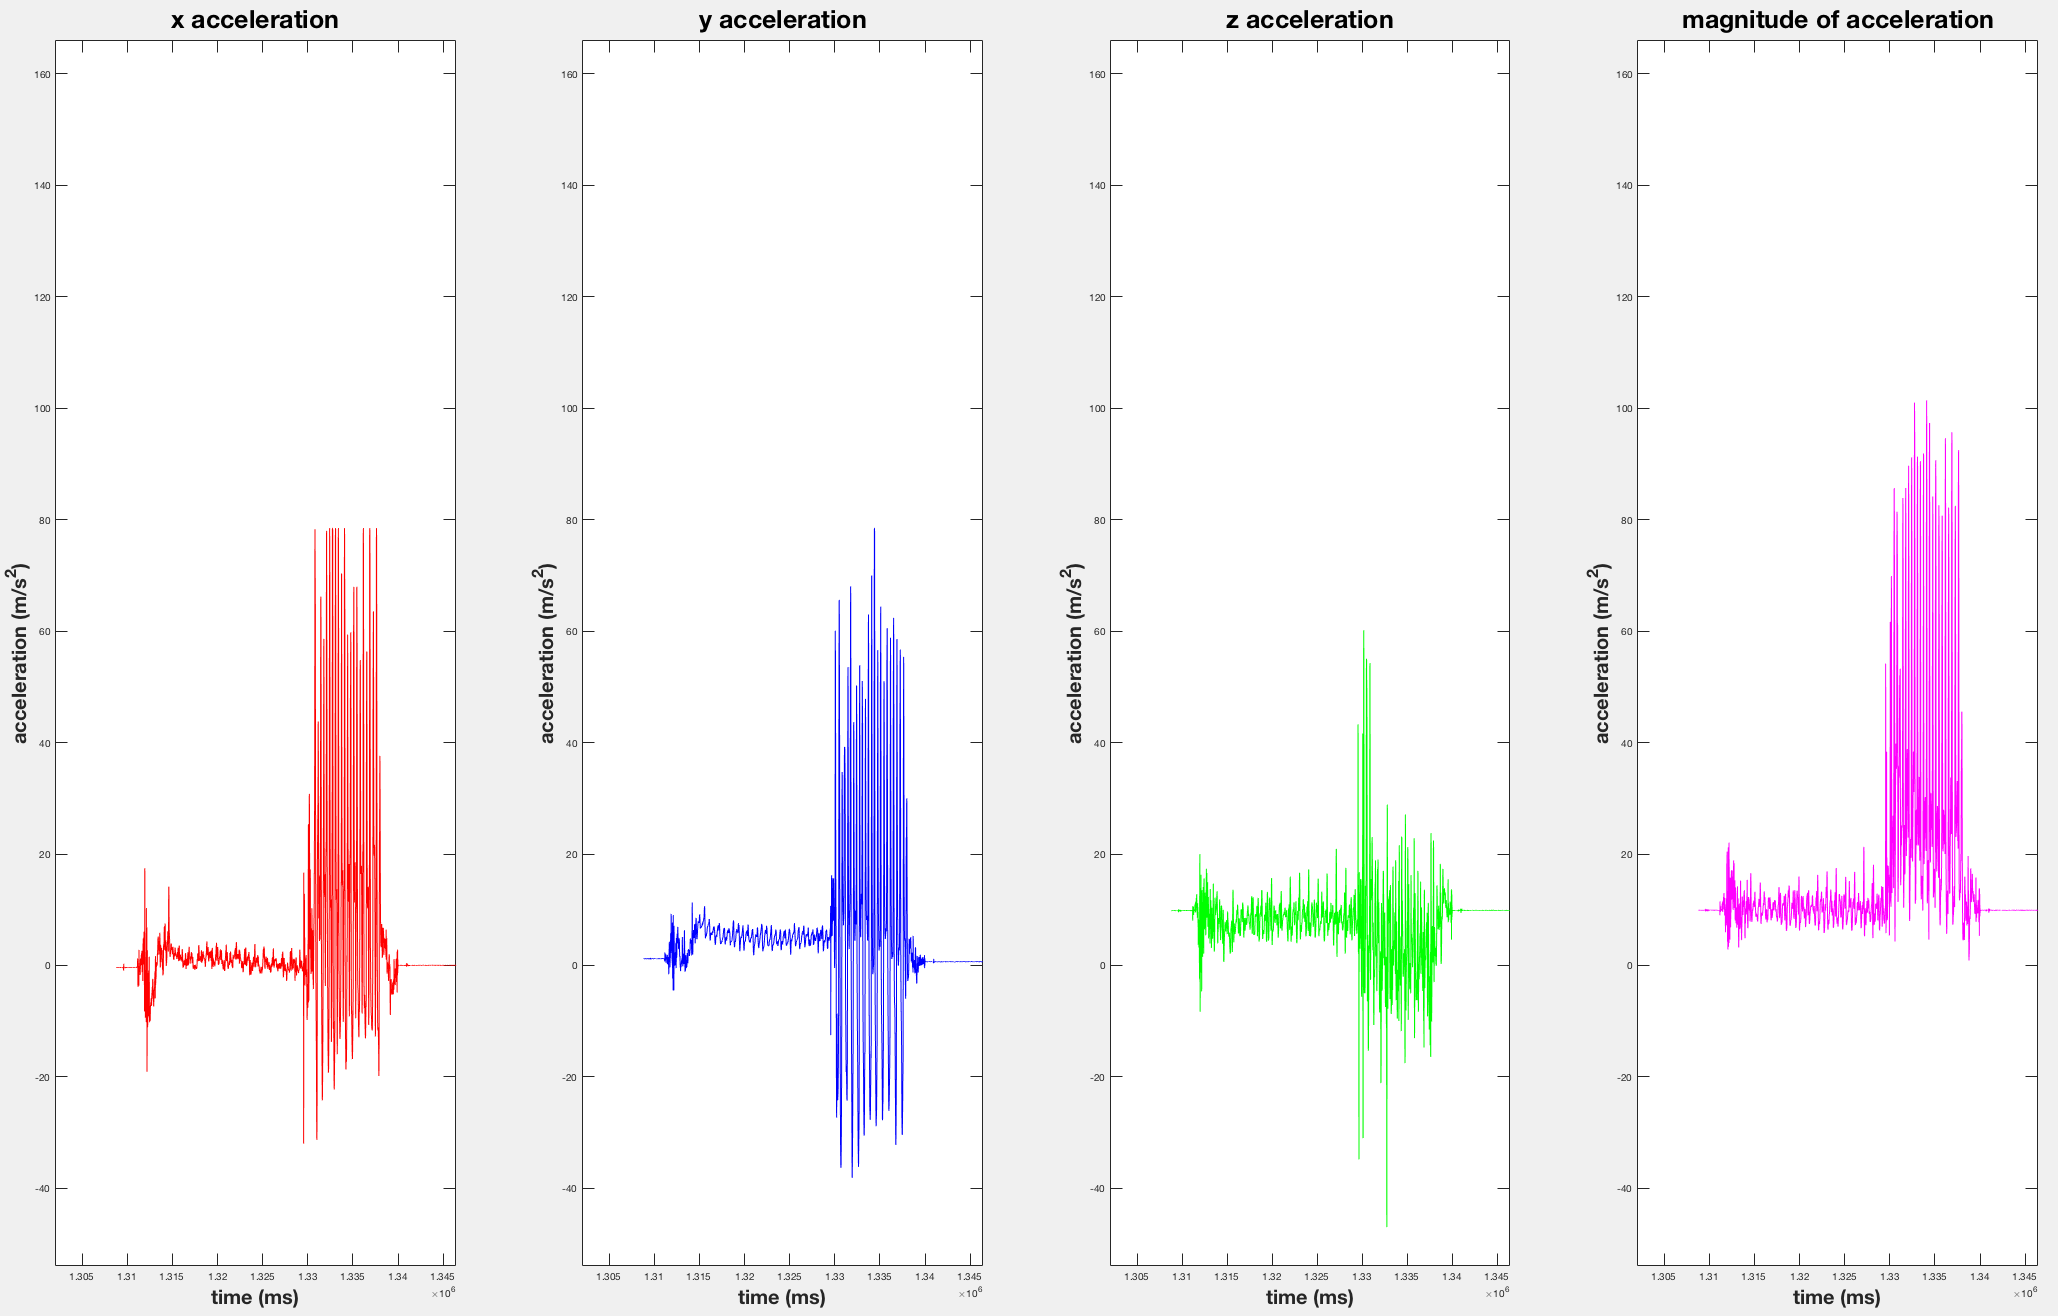
\includegraphics[width=1.0\columnwidth]{pos_acc_separated.png}
\caption{The X, Y, Z and magnitude of acceleration, respectively, from one simulated theft instance.}
\label{fig:simtheft}
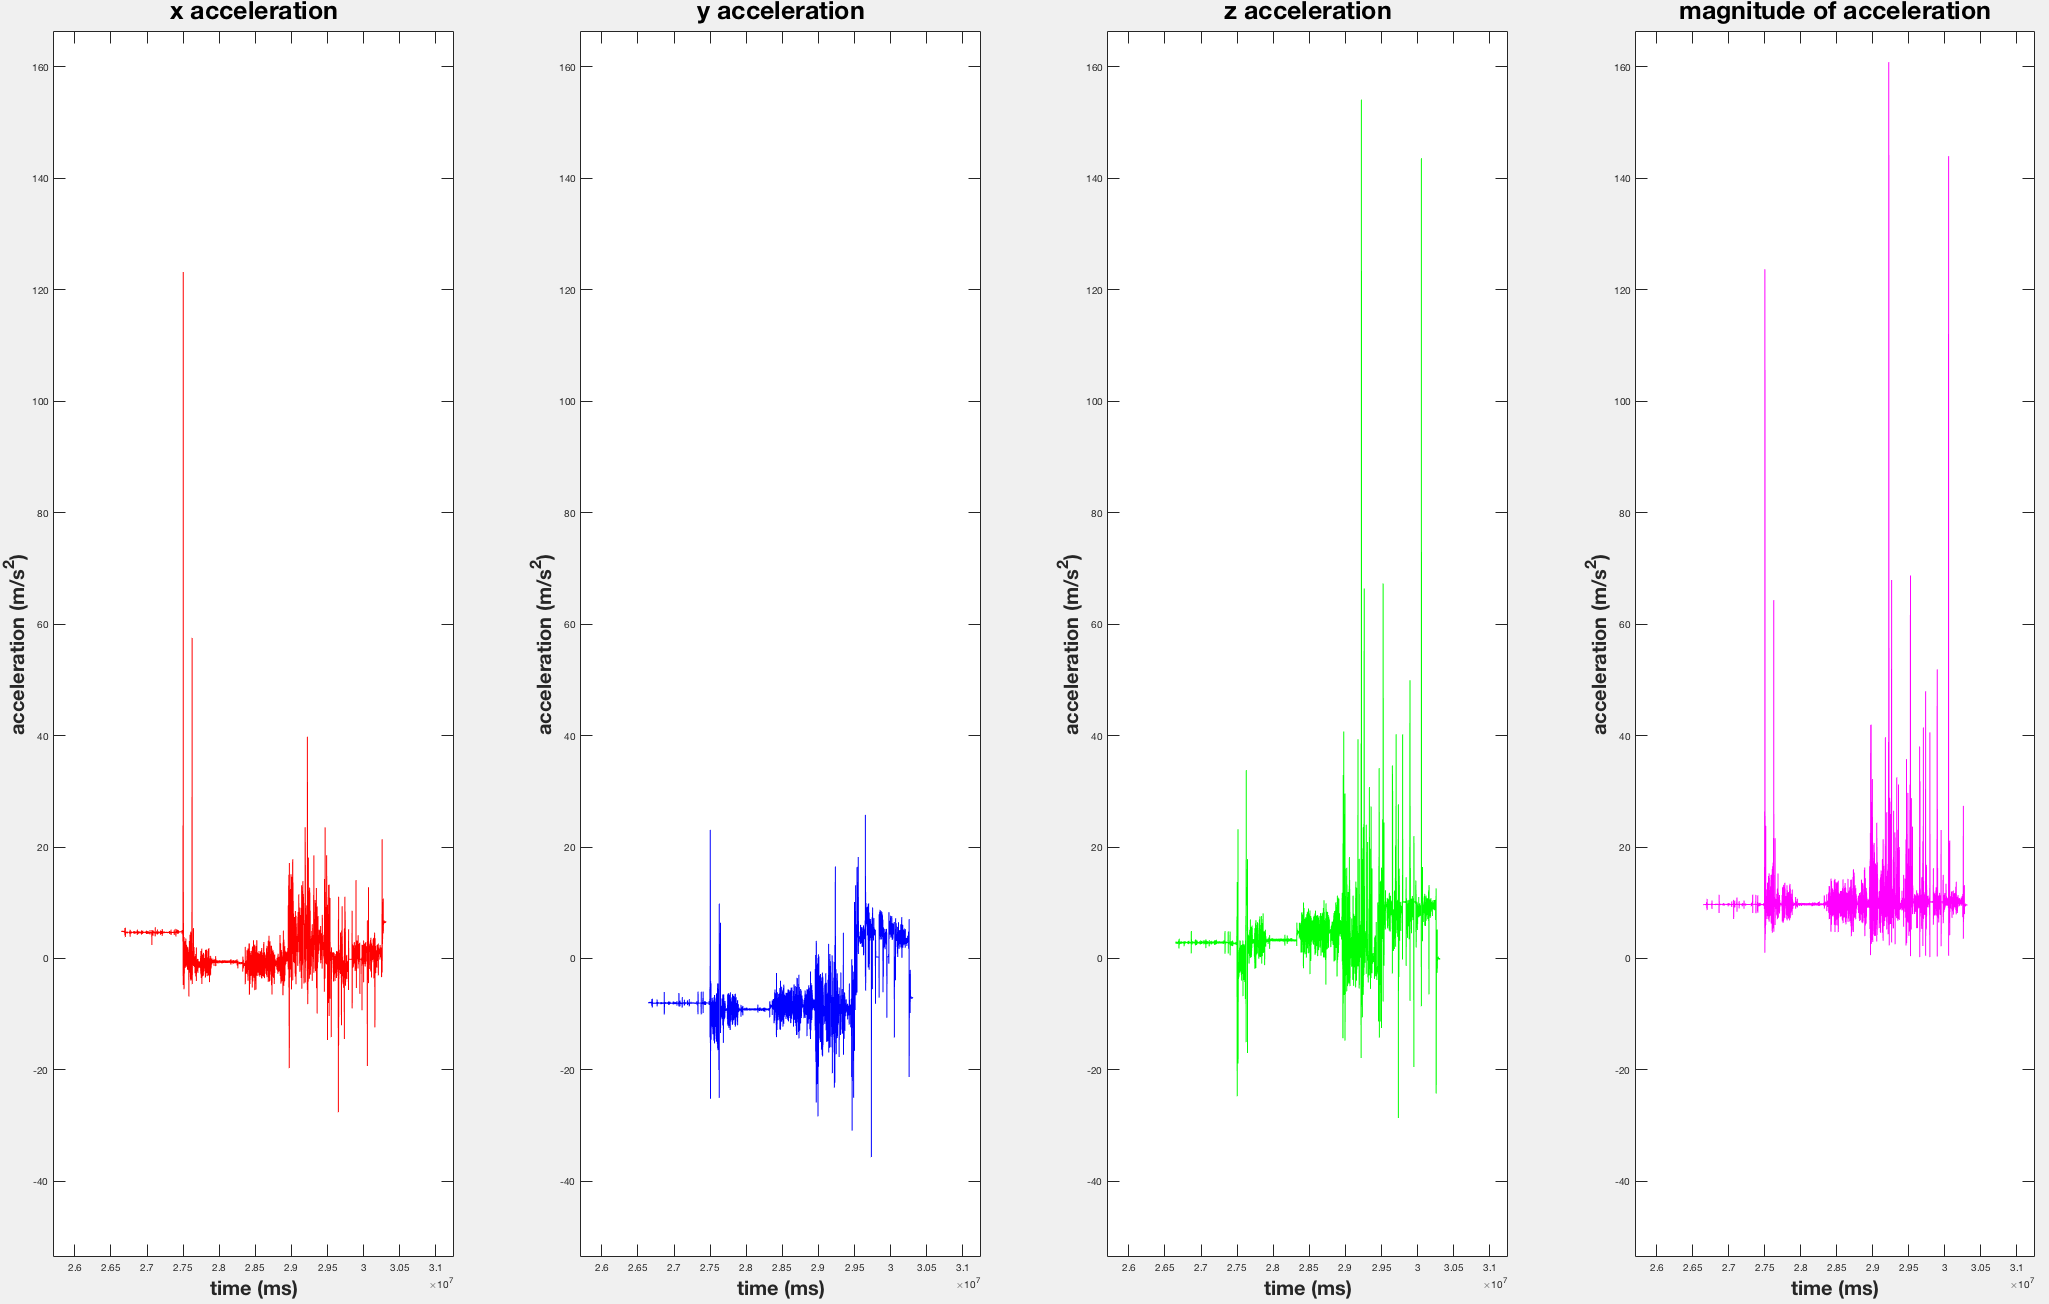
\includegraphics[width=1.0\columnwidth]{neg_acc_separated.png}
\caption{The X, Y, Z and magnitude of acceleration, respectively, during normal usage at an arbitrary time period.}
\end{figure}




\subsubsection{Field Study}
We performed a field study to gather data from ordinary smartphone users
during their everyday life.
% We obtained approval from the University of California, Berkeley IRB (Institutional Review Board) for this study. 
We obtained approval from our university IRB (Institutional Review Board) for this study. 
The study was conducted in a metropolitan area from September to December 2016.
% The study was conducted in the Bay Area of the United States from September to December 2016.
None of the participants experienced a phone theft during the study interval,
so we were able to use the accelerometer data collected from the user study as negative samples for our machine learning algorithms (i.e., instances of non-theft activity).

We posted a recruitment advertisement on the Craigslist in September 2016. 
% We posted a recruitment advertisement on the Craigslist under the SF Bay Area `jobs et cetera' category in September 2016. 
We only recruited participants who used an Android smartphone with version 5.0 and above.
After obtaining their consent, we installed our data collection application on their phones and collected data for a three-week period.
The application ran in the background and collected accelerometer sensor readings continuously, 24 hours a day.
We contacted participants weekly to make sure their phones were functioning correctly and troubleshoot any data collection issues.
Each participant was paid \$150 for their participation.

The study was divided across 3 rounds; each round lasted 3 consecutive weeks. 
A total of 55 participants were recruited, and
53 out of the 55 subjects completed the study. 
In the first round, 2 of the 18 participants did not complete the study.
Detailed demographic information about the participants of this user study is listed in Table~\ref{tbl:demographics}.
In aggregate they used 21 different smartphone models from 6 different manufacturers, including 2 subjects using Nexus 5X and 3 using Nexus 5, 6, 6P phones.
We asked them how they typically carried their phone, when it wasn't in their hand; 33 reported keeping it in their pocket, 9 in their purse, 12 in multiple locations (e.g., pocket or purse, pocket or backpack), and 1 did not respond.
Therefore, we believe we observed a wide variety of behaviors and devices in this study.

\begin{table}[H]
\centering
\begin{tabular}{rrrrrr}
\hline
      & Male & Female & Age 20--29 & 30--39 & 40+ \\ \hline
R1    & 5    & 11     & 8         & 6     & 2   \\
R2    & 10   & 8      & 7         & 7     & 4   \\
R3    & 11   & 8      & 9         & 4     & 6   \\
Total & 26   & 27     & 24        & 17    & 12  \\ \hline
\end{tabular}
\caption{Demographic Info of the User Study}
\label{tbl:demographics}
\end{table}




\subsection{Feature Extraction}
\label{s:features}

Our theft scenarios all involve a sudden movement of the phone, which causes a large acceleration.
Therefore, as a first filtering step, we filter the data to focus on times near when a large motion occurs.
In particular, our classifier is activated when the magnitude of acceleration $M$ exceeds~$40 m/s^2$.
We extract a one-second window before the activation time and a $n$-second window after the activation time, compute features on each of these windows, and use them for classification.
We vary $n$ from 1 to 7 to obtain the best classification accuracy.
We chose a threshold of~$40 m/s^2$ as all of our simulated thefts experienced accelerations exceeding that threshold when the phone was initially grabbed by the thief.

We first identified 16 candidate features, 8 features for each of the two windows.
In particular, we computed the minimum, maximum, mean, standard deviation, root mean square, arc length, product of arc length and standard deviation, and mean absolute value, each computed on the magnitude values ($M$) within the window.
We chose to only compute these features on the magnitude of the acceleration, and not the $X$, $Y$, and $Z$ components, because the magnitude is non-directional thus more robust to changes in the orientation of the phone. 
We then visualized the distribution of these features for the two classes and applied feature selection techniques to choose a subset of features that yield good performance.
We removed the minimum and mean absolute value from the feature list because removing them did not affect the performance of the classifiers. 
As a result, we extract a 12-dimensional feature vector, 6 features from the before-window and 6 from the after-window, every time the detector is triggered.

Let $M_1,\dots,M_k$ denote the time series of acceleration magnitudes within the window.
The features are computed as follows:
\begin{itemize}
\item \emph{Maximum}: the maximum value of the magnitude within the window, i.e., $\max(M_1,\dots,M_k)$.
\item \emph{Mean}: the average value of magnitude in a window, i.e., $(M_1+\dots + M_k)/k$.
\item \emph{Standard deviation}: the standard deviation of magnitude values in a window.
\item \emph{Root mean square}: the rms of magnitude values in a window, i.e., $(M_1^2 + \dots + M_k^2)^{1/2}/k^{1/2}$.
\item \emph{Arc length}: the average of the absolute differences between all adjacent magnitude values in a window, i.e., $(|M_2-M_1| + |M_3-M_2| + \dots + |M_k-M_{k-1}|)/(k-1)$.
Intuitively, this captures the average of the first derivative of the acceleration.
\item \emph{Product of arc length and standard deviation}: the product of the two feature values.
\end{itemize}

Because the accelerometer sensor reports readings in the same units on all Android phones, and because our features are relatively simple, we believe these features capture fundamental, device-independent characteristics of the motion rather than anything specific to the particular device used to capture the data.

We obtain 60 positive instances from the 60 simulated thefts.
After applying the~$40 m/s^2$ threshold, we obtain approximately approximately 248000 negative samples from the data collected in the field study. 
We then apply boolean classification techniques to this data set.


% \begin{figure}[t]
% 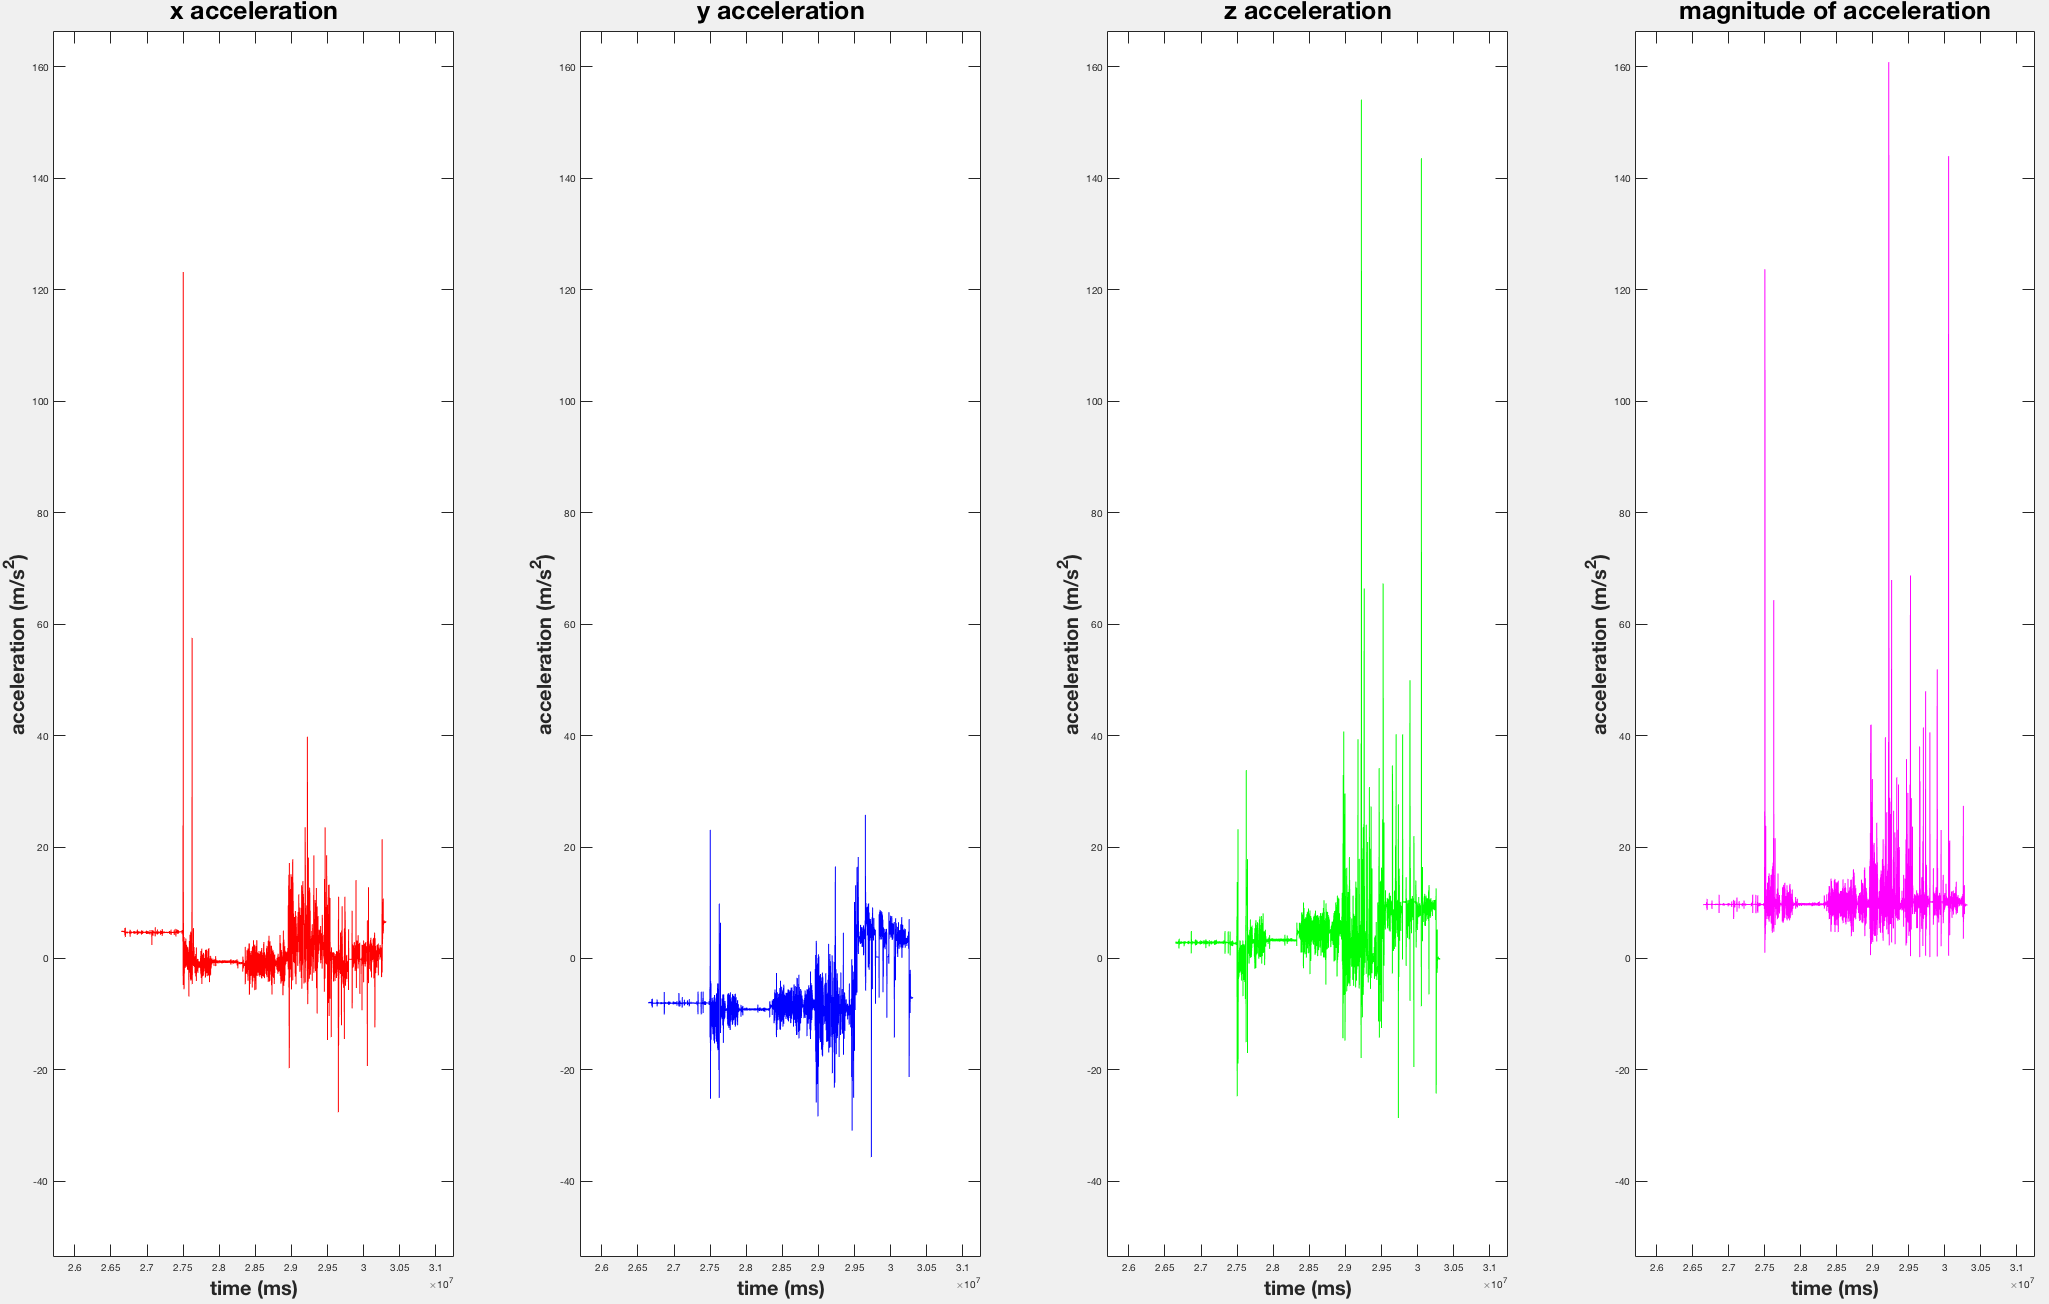
\includegraphics[width=1.0\columnwidth]{neg_acc_separated.png}
% \caption{The X, Y, Z and magnitude of acceleration, respectively, during normal usage at an arbitrary time period.}
% \end{figure}



\subsection{Machine Learning Algorithms}
We evaluate three standard machine learning algorithms: linear SVM, logistic regression and random forests.
Because we have many more negative samples than positive ones, we tried different settings for class weights to weight positive instances more highly than negative ones.
We also evaluated different window sizes for the after-window.
We found that a 2-second after-window yielded better accuracy than a 1-second after-window, and larger window sizes did not offer much improvement.
Therefore, all of our experiments use a 1-second before-window and a 2-second after-window.
We evaluated the classifiers using 10-fold cross validation on the entire dataset, which consists of 60 positive samples and approximately 248,000 negative samples. 



\section{Results}
Among the three classifiers, logistic regression performs the best.
Confusion matrices for logistic regression, random forests, and a linear SVM
are shown in Table~\ref{fig:cmat}.
The logistic regression classifier has a false positive rate of 0.07\%, which means that on average users receive 1 false alarm every week, and a true positive rate of 100\%.
The random forests classifier has an even lower false positive rate (less than one false alarm per month),
but it only detects half of thefts.
The linear SVM's false positive rate is too high for our purposes.


\begin{table}[t]
\centering
\begin{tabular}{@{}lll@{}}
\toprule
              & Predicted Negative & Predicted Positive \\ \midrule
True Negative & 248223             & 170                \\
True Positive & 0                  & 60                 \\ \bottomrule
\end{tabular}

\begin{tabular}{@{}lll@{}}
\toprule
              & Predicted Negative & Predicted Positive \\ \midrule
True Negative & 248360             & 33                 \\
True Positive & 32                 & 28                 \\ \bottomrule
\end{tabular}

\begin{tabular}{@{}lll@{}}
\toprule
              & Predicted Negative & Predicted Positive \\ \midrule
True Negative & 246522             & 1871               \\
True Positive & 42                 & 18                 \\ \bottomrule
\end{tabular}
\caption{Confusion matrices for a logistic regression classifier (at top; with class weights 1:200), random forests classifier (middle; class weights 1:5000), and a linear SVM classifier (bottom; class weights 1:1000).}
\label{fig:cmat}
\end{table}

% \begin{table}[t]
% \centering
% \begin{tabular}{@{}lll@{}}
% \toprule
%               & Predicted Negative & Predicted Positive \\ \midrule
% True Negative & 248223             & 170                \\
% True Positive & 0                  & 60                 \\ \bottomrule
% \end{tabular}
% \caption{Confusion matrix for a logistic regression classifier trained
% with class weights set to 1:200.}
% \label{fig:logistic}
% \end{table}

% \begin{table}[t]
% \centering
% \begin{tabular}{@{}lll@{}}
% \toprule
%               & Predicted Negative & Predicted Positive \\ \midrule
% True Negative & 248360             & 33                 \\
% True Positive & 32                 & 28                 \\ \bottomrule
% \end{tabular}
% \caption{Confusion matrix for a random forests classifier trained with
% class weights set to 1:5000.}
% \label{fig:rf}

% \end{table}

% \begin{table}[t]
% \centering
% \begin{tabular}{@{}lll@{}}
% \toprule
%               & Predicted Negative & Predicted Positive \\ \midrule
% True Negative & 246522             & 1871               \\
% True Positive & 42                 & 18                 \\ \bottomrule
% \end{tabular}
% \caption{Confusion matrix for a linear SVM classifier trained with
% class weights set to 1:1000.}
% \label{fig:svm}
% \end{table}


To get a better understanding of why our classifier is successful,
we computed feature rankings to find the most predictive features.
For logistic regression, we use standardized coefficients as the feature importance score:
the score for feature $i$ is $|\alpha_i| \cdot \sigma_i$, where $\alpha_i$ is the coefficient for feature $i$ in the logistic regression model and $\sigma_i$ is the standard deviation of feature $i$ in the training set.
The feature importance scores for the logistic regression classifier are listed in Table~\ref{tbl:importance-lr}.
The most discriminative features are
the maximum of the before-window,
the product of arc length and standard deviation of the after-window,
and the arc length of the before-window.
Plotting a histogram of feature values (see Figures~\ref{fig:beforehist} and \ref{fig:afterhist}), we can see that those features do appear to provide good discrimination.


\begin{table}[t]
\centering
\begin{tabular}{@{}ll@{}}
\toprule
Feature                & Feature Importance \\ \midrule
Maximum (b)            & 2.73319487         \\
Arc length * SD (a)    & 2.69540663         \\
Arc length (b)         & 1.18427357         \\
Root mean square (a)   & 0.937781183        \\
Mean (a)               & 0.880738694        \\
Standard deviation (a) & 0.666823228        \\
Standard deviation (b) & 0.477534932        \\
Arc length (a)         & 0.273227115        \\
Maximum (a)            & 0.0580951517       \\
Arc length * SD (b)    & 0.0470492037       \\
Root mean square (b)   & 0.0143829911       \\
Mean (b)               & 0.0129842047       \\ \bottomrule
\end{tabular}
\caption{Feature importances for logistic regression. (b) denotes the features extracted from the 1s window before the 40-spike; (a) denotes the features extracted from the 2s window after the 40-spike.}
\label{tbl:importance-lr}
\end{table}

We also rank the features for the random forests classifier using scikit-learn's feature importance score, which estimates the relative importance of the features by computing the expected fraction of the samples they contribute to. 
Thus the higher in the tree, the more important the feature is~\cite{sklearn:rfdoc}. 
% 0.04751106, 0.0080411, 0.02881483, 0.01533719, 0.02245781, 0.03309431, 0.12388036, 0.20288397, 0.16426152, 0.21908845, 0.05162059, 0.0830088.
The resulting feature importance scores for the random forests classifier are listed in Table~\ref{tbl:importance-rf}.

% Another way to visulize the representative features is to plot a histogram of dataset and to see which features can better seperate the positive and negative data points, as shown in Figures 1 and 2.

\begin{table}[t]
\centering
\begin{tabular}{@{}ll@{}}
\toprule
Feature                & Feature Importance \\ \midrule
Root mean square (a)   & 0.21908845         \\
Mean (a)               & 0.20288397         \\
Standard deviation (a) & 0.16426152         \\
Maximum (a)            & 0.12388036         \\
Arc length * SD (a)    & 0.0830088          \\
Arc length (a)         & 0.05162059         \\
Maximum (b)            & 0.04751106         \\
Arc length * SD (b)    & 0.03309431         \\
Standard deviation (b) & 0.02881483         \\
Arc length (b)         & 0.02245781         \\
Root mean square (b)   & 0.01533719         \\
Mean (b)               & 0.0080411          \\ \bottomrule
\end{tabular}
\caption{Feature importances for random forests. (b) denotes the features extracted from the 1s window before the 40-spike; (a) denotes the features extracted from the 2s window after the 40-spike.}
\label{tbl:importance-rf}
\end{table}


% \begin{figure*}[t]

% \begin{center}
% \begin{minipage}
% 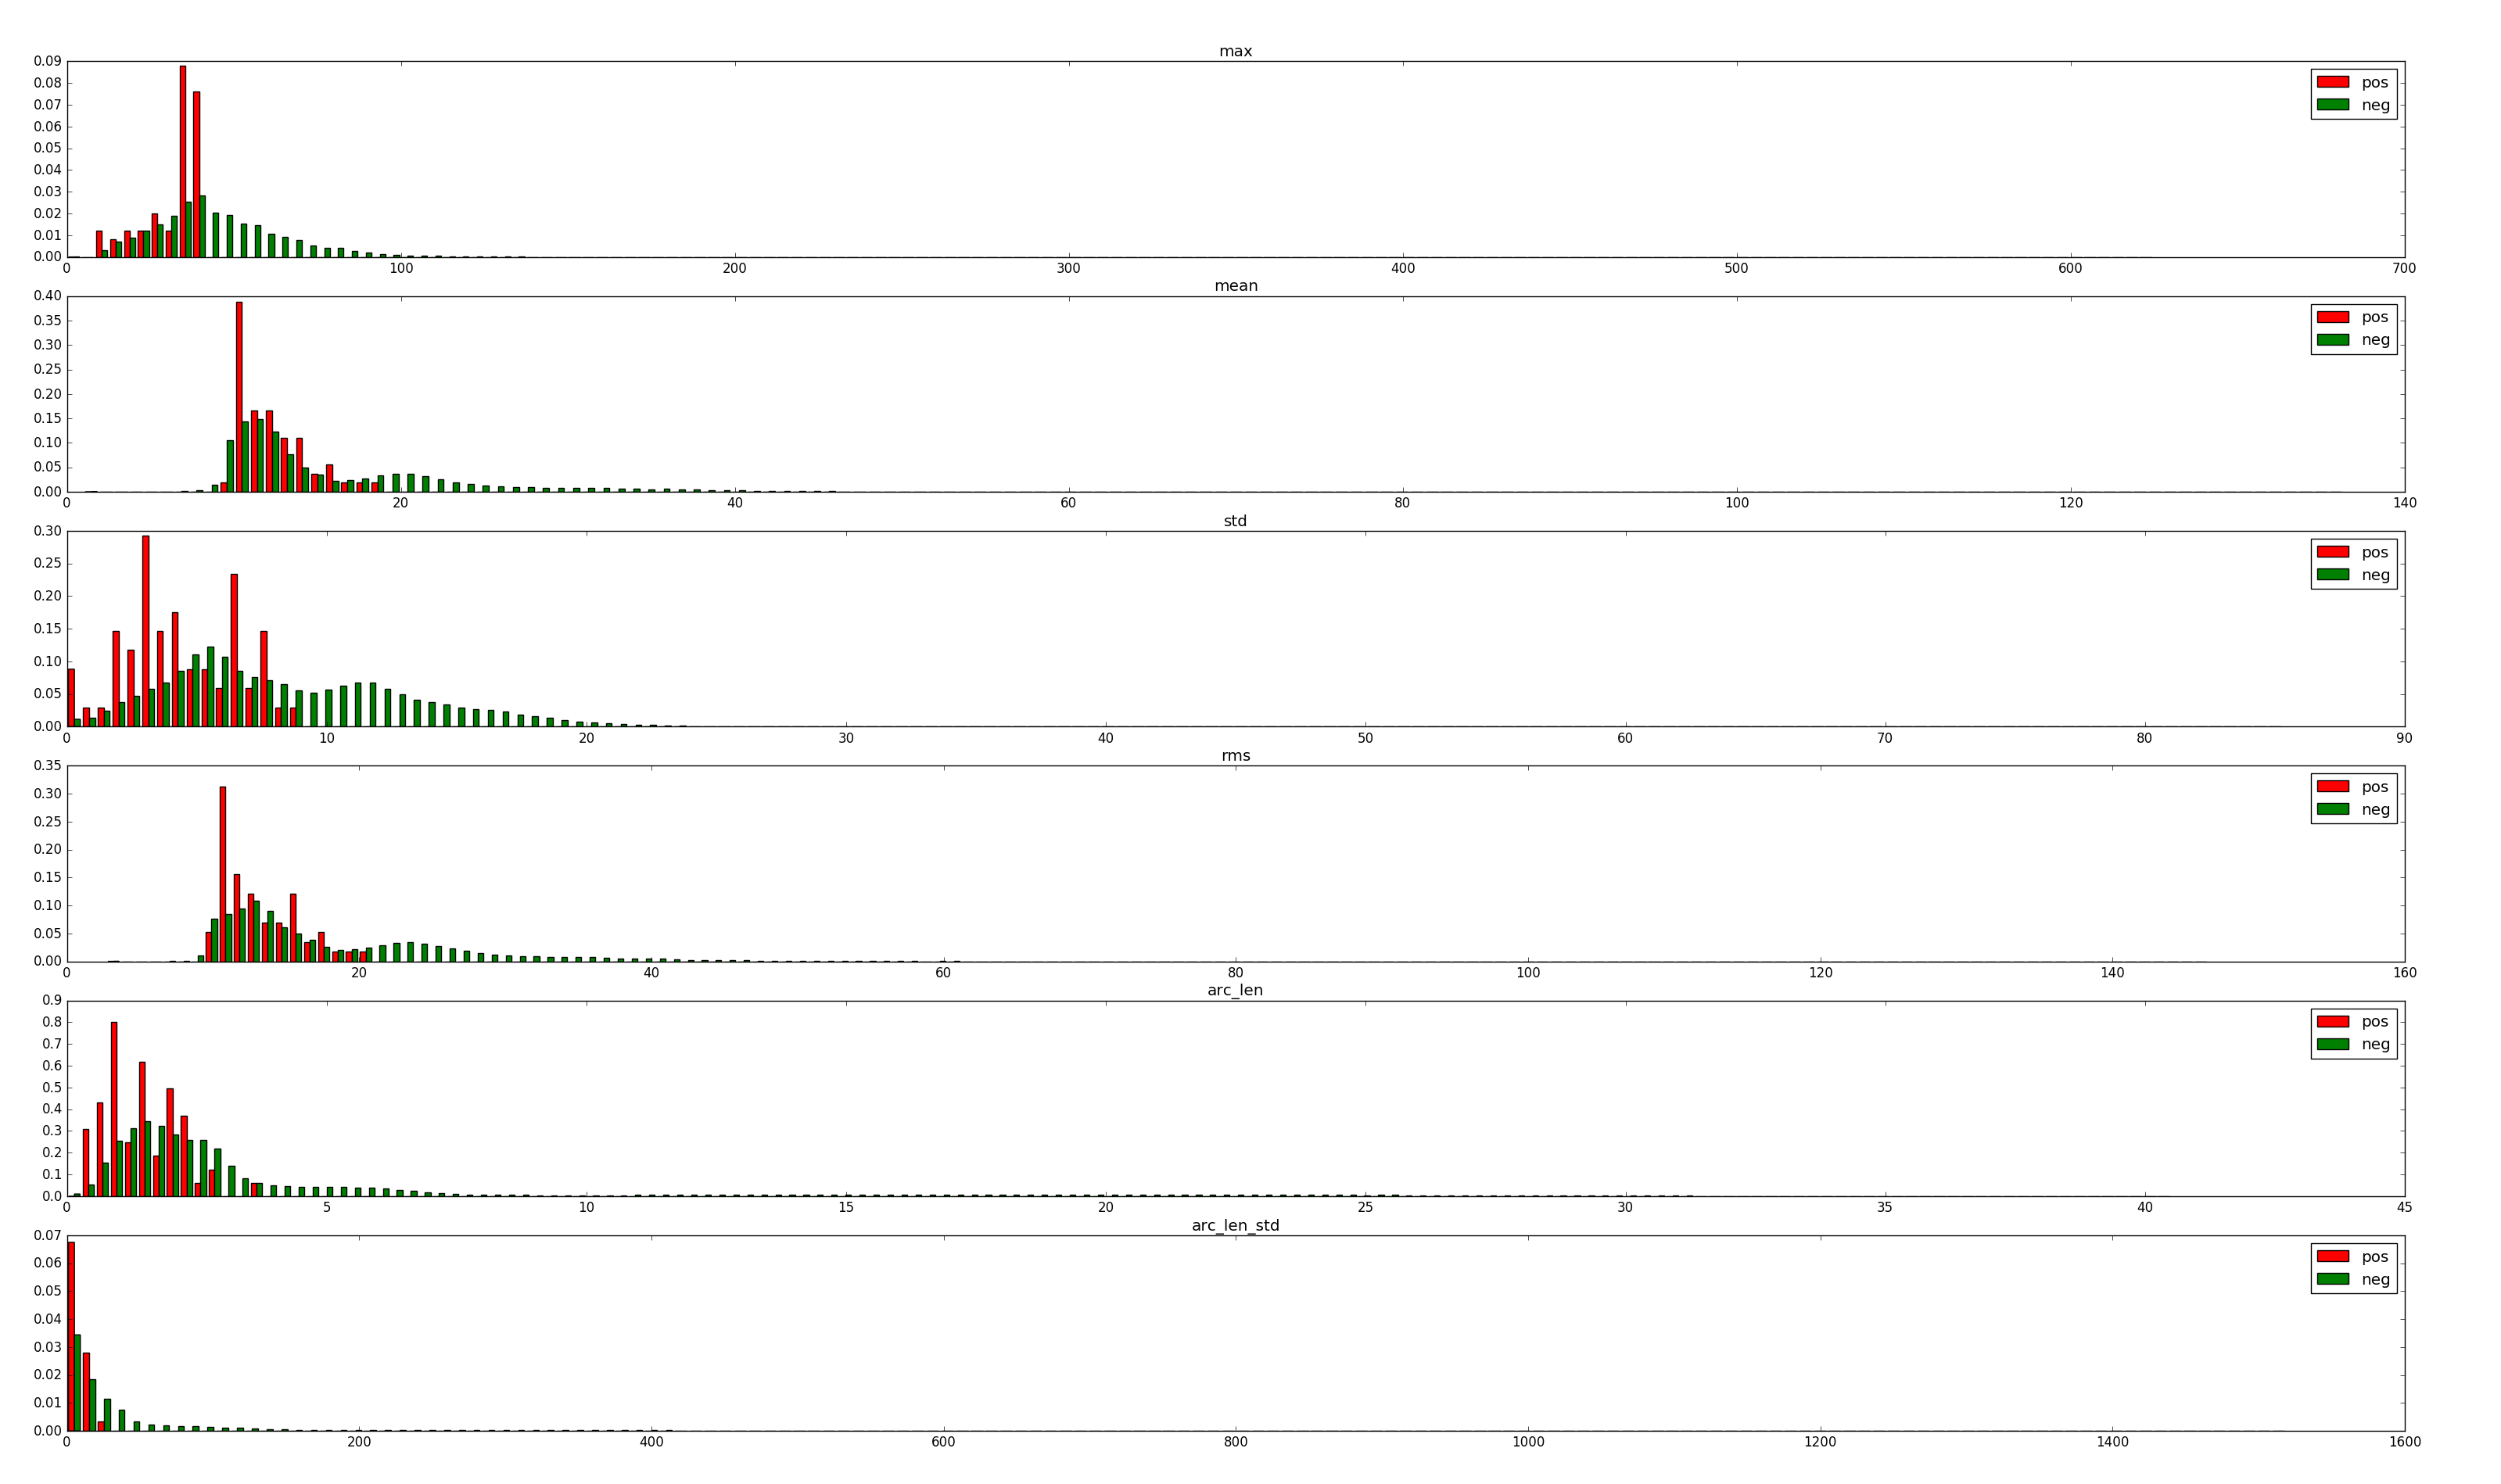
\includegraphics[width=\textwidth]{hist_features_before_win_size_1_2.png}
% \end{minipage}
% \end{center}
% \caption{Histogram for each of the 6 features for the 1-second window before the~$40 m/s^2$ spike.  The features are listed in the order presented in Section~\ref{s:features}, e.g., the top histogram is for the maximum.  Red bars indicate thefts, and green bars indicate non-theft windows.}
% \label{fig:beforehist}
% \begin{center}
% \begin{minipage}
% 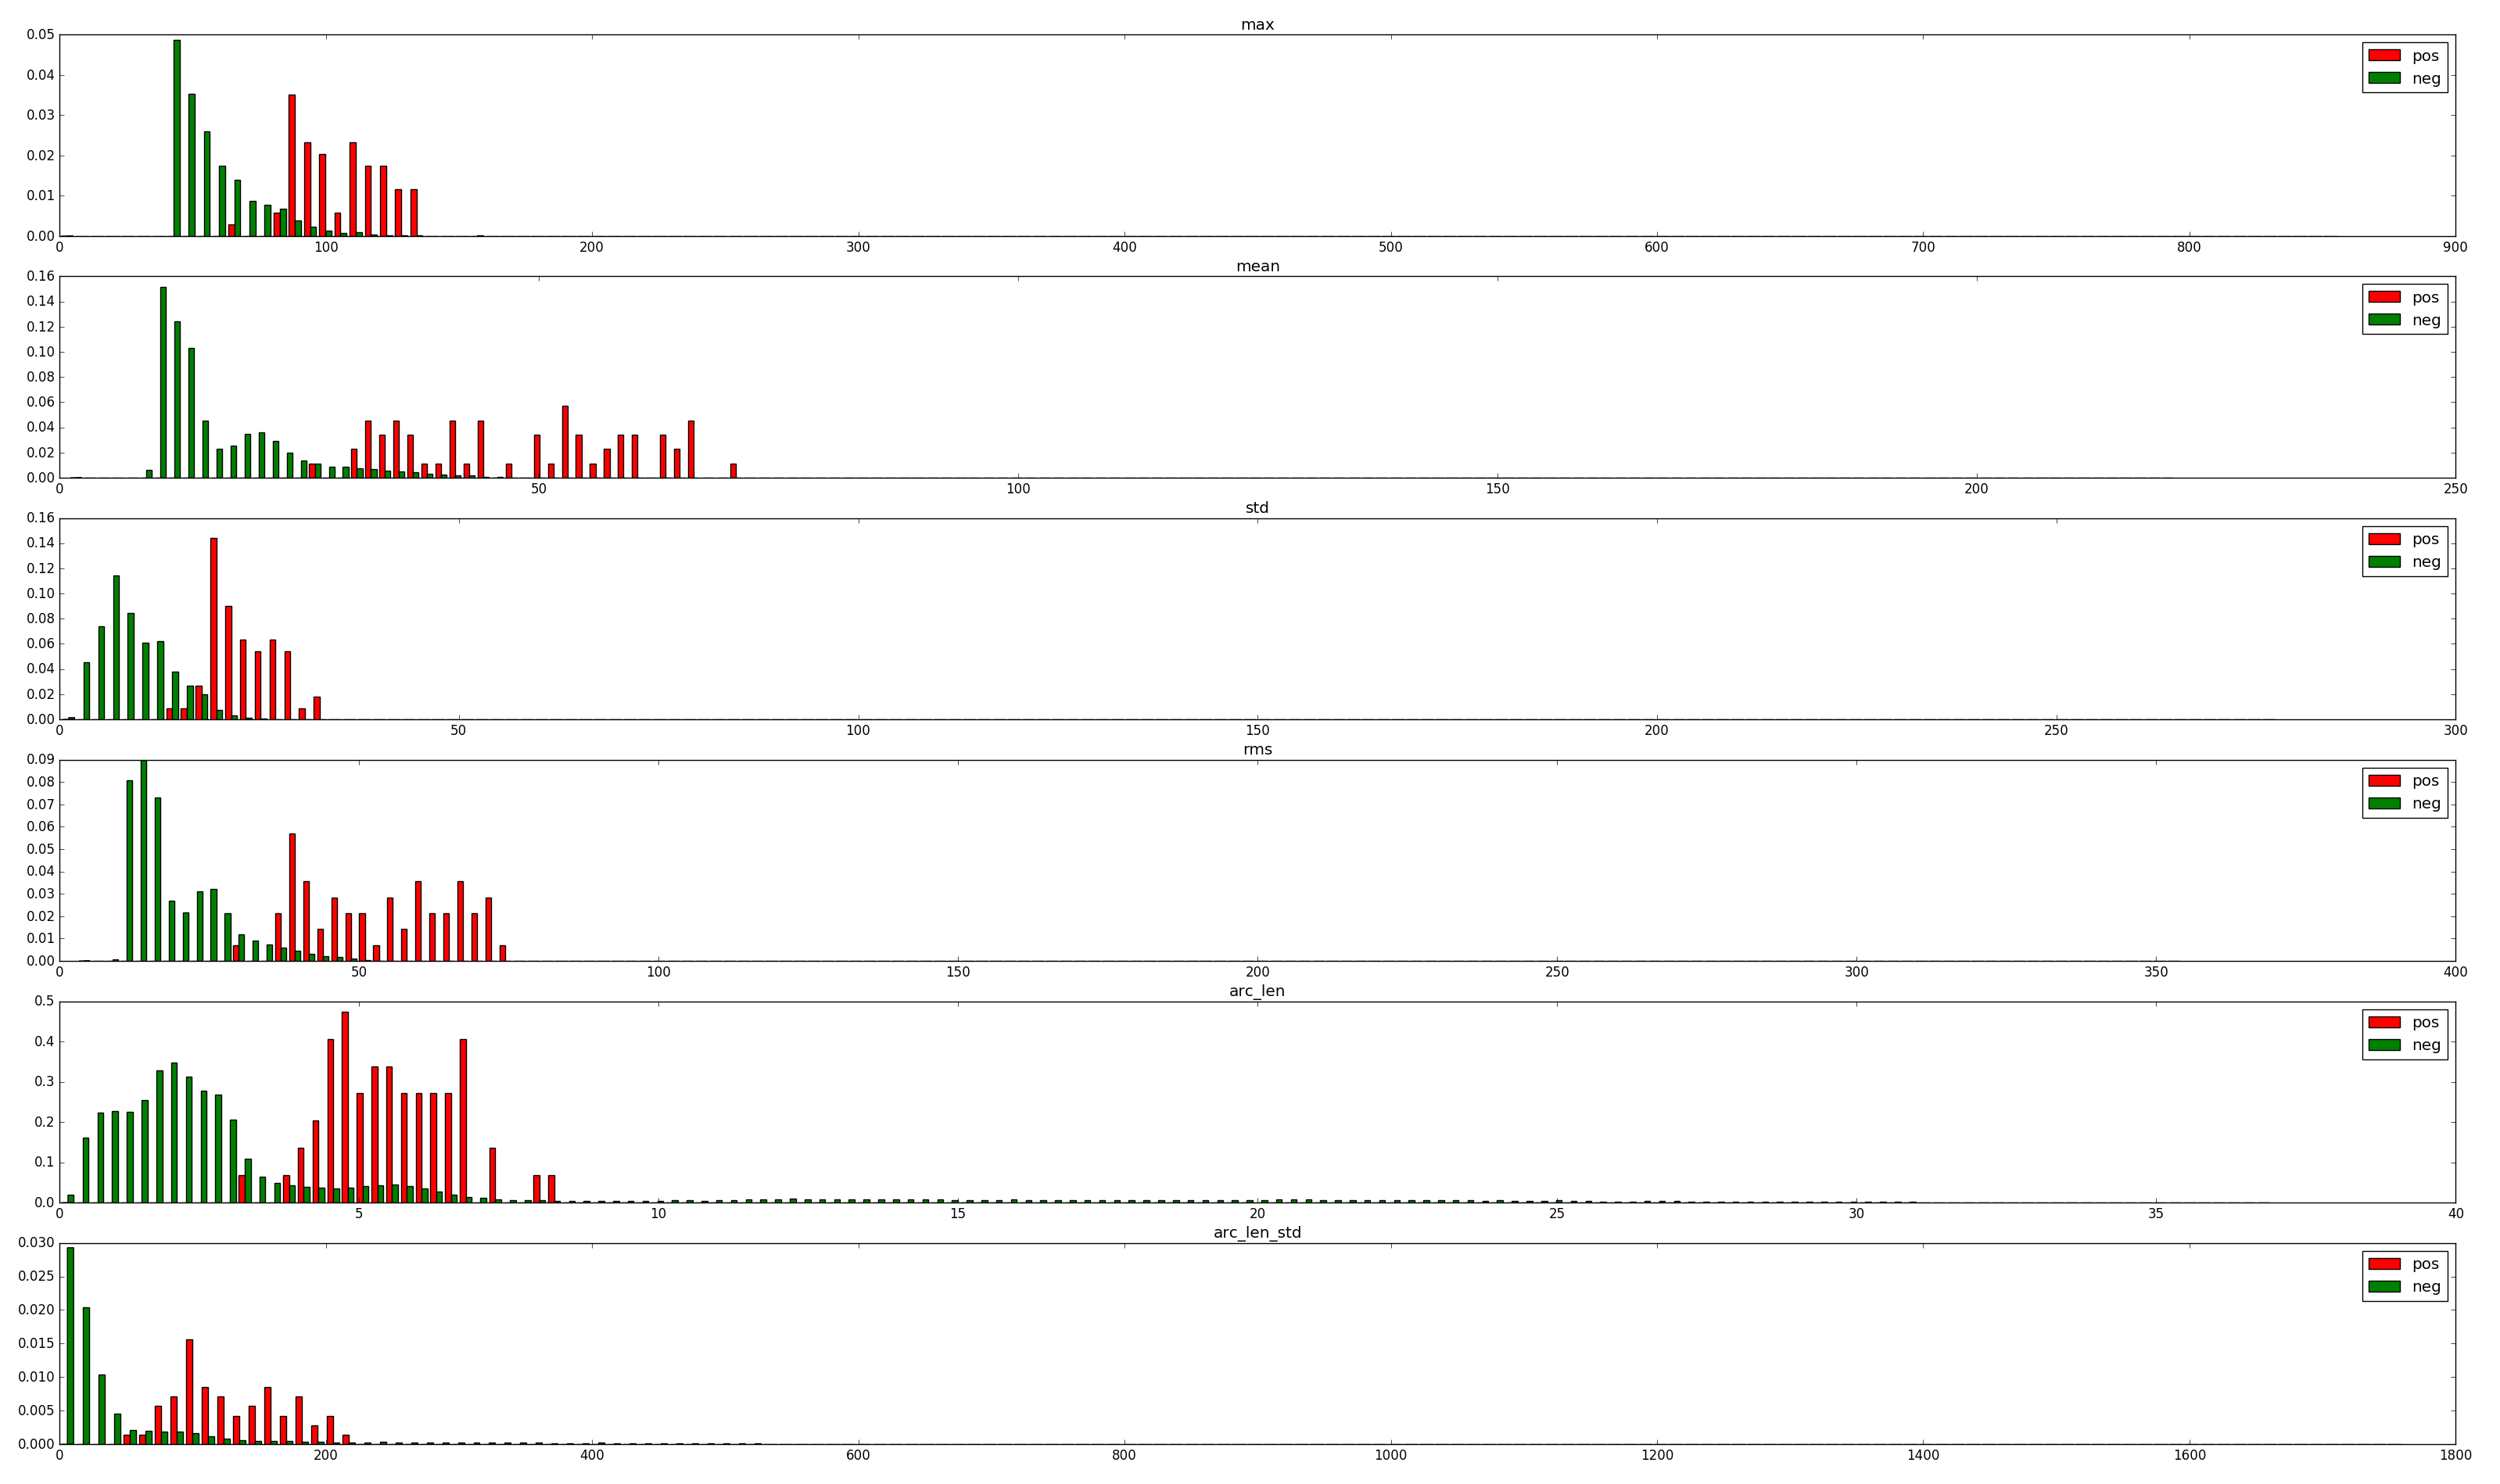
\includegraphics[width=\textwidth]{hist_features_after_win_size_1_2.png}
% \end{minipage}
% \end{center}
% \caption{Histogram of feature values in the 2-second window after the~$40 m/s^2$ spike.}
% \label{fig:afterhist}

% \end{figure*}


\begin{figure*}[t]
\centering
\begin{minipage}[t]{0.4\textwidth}
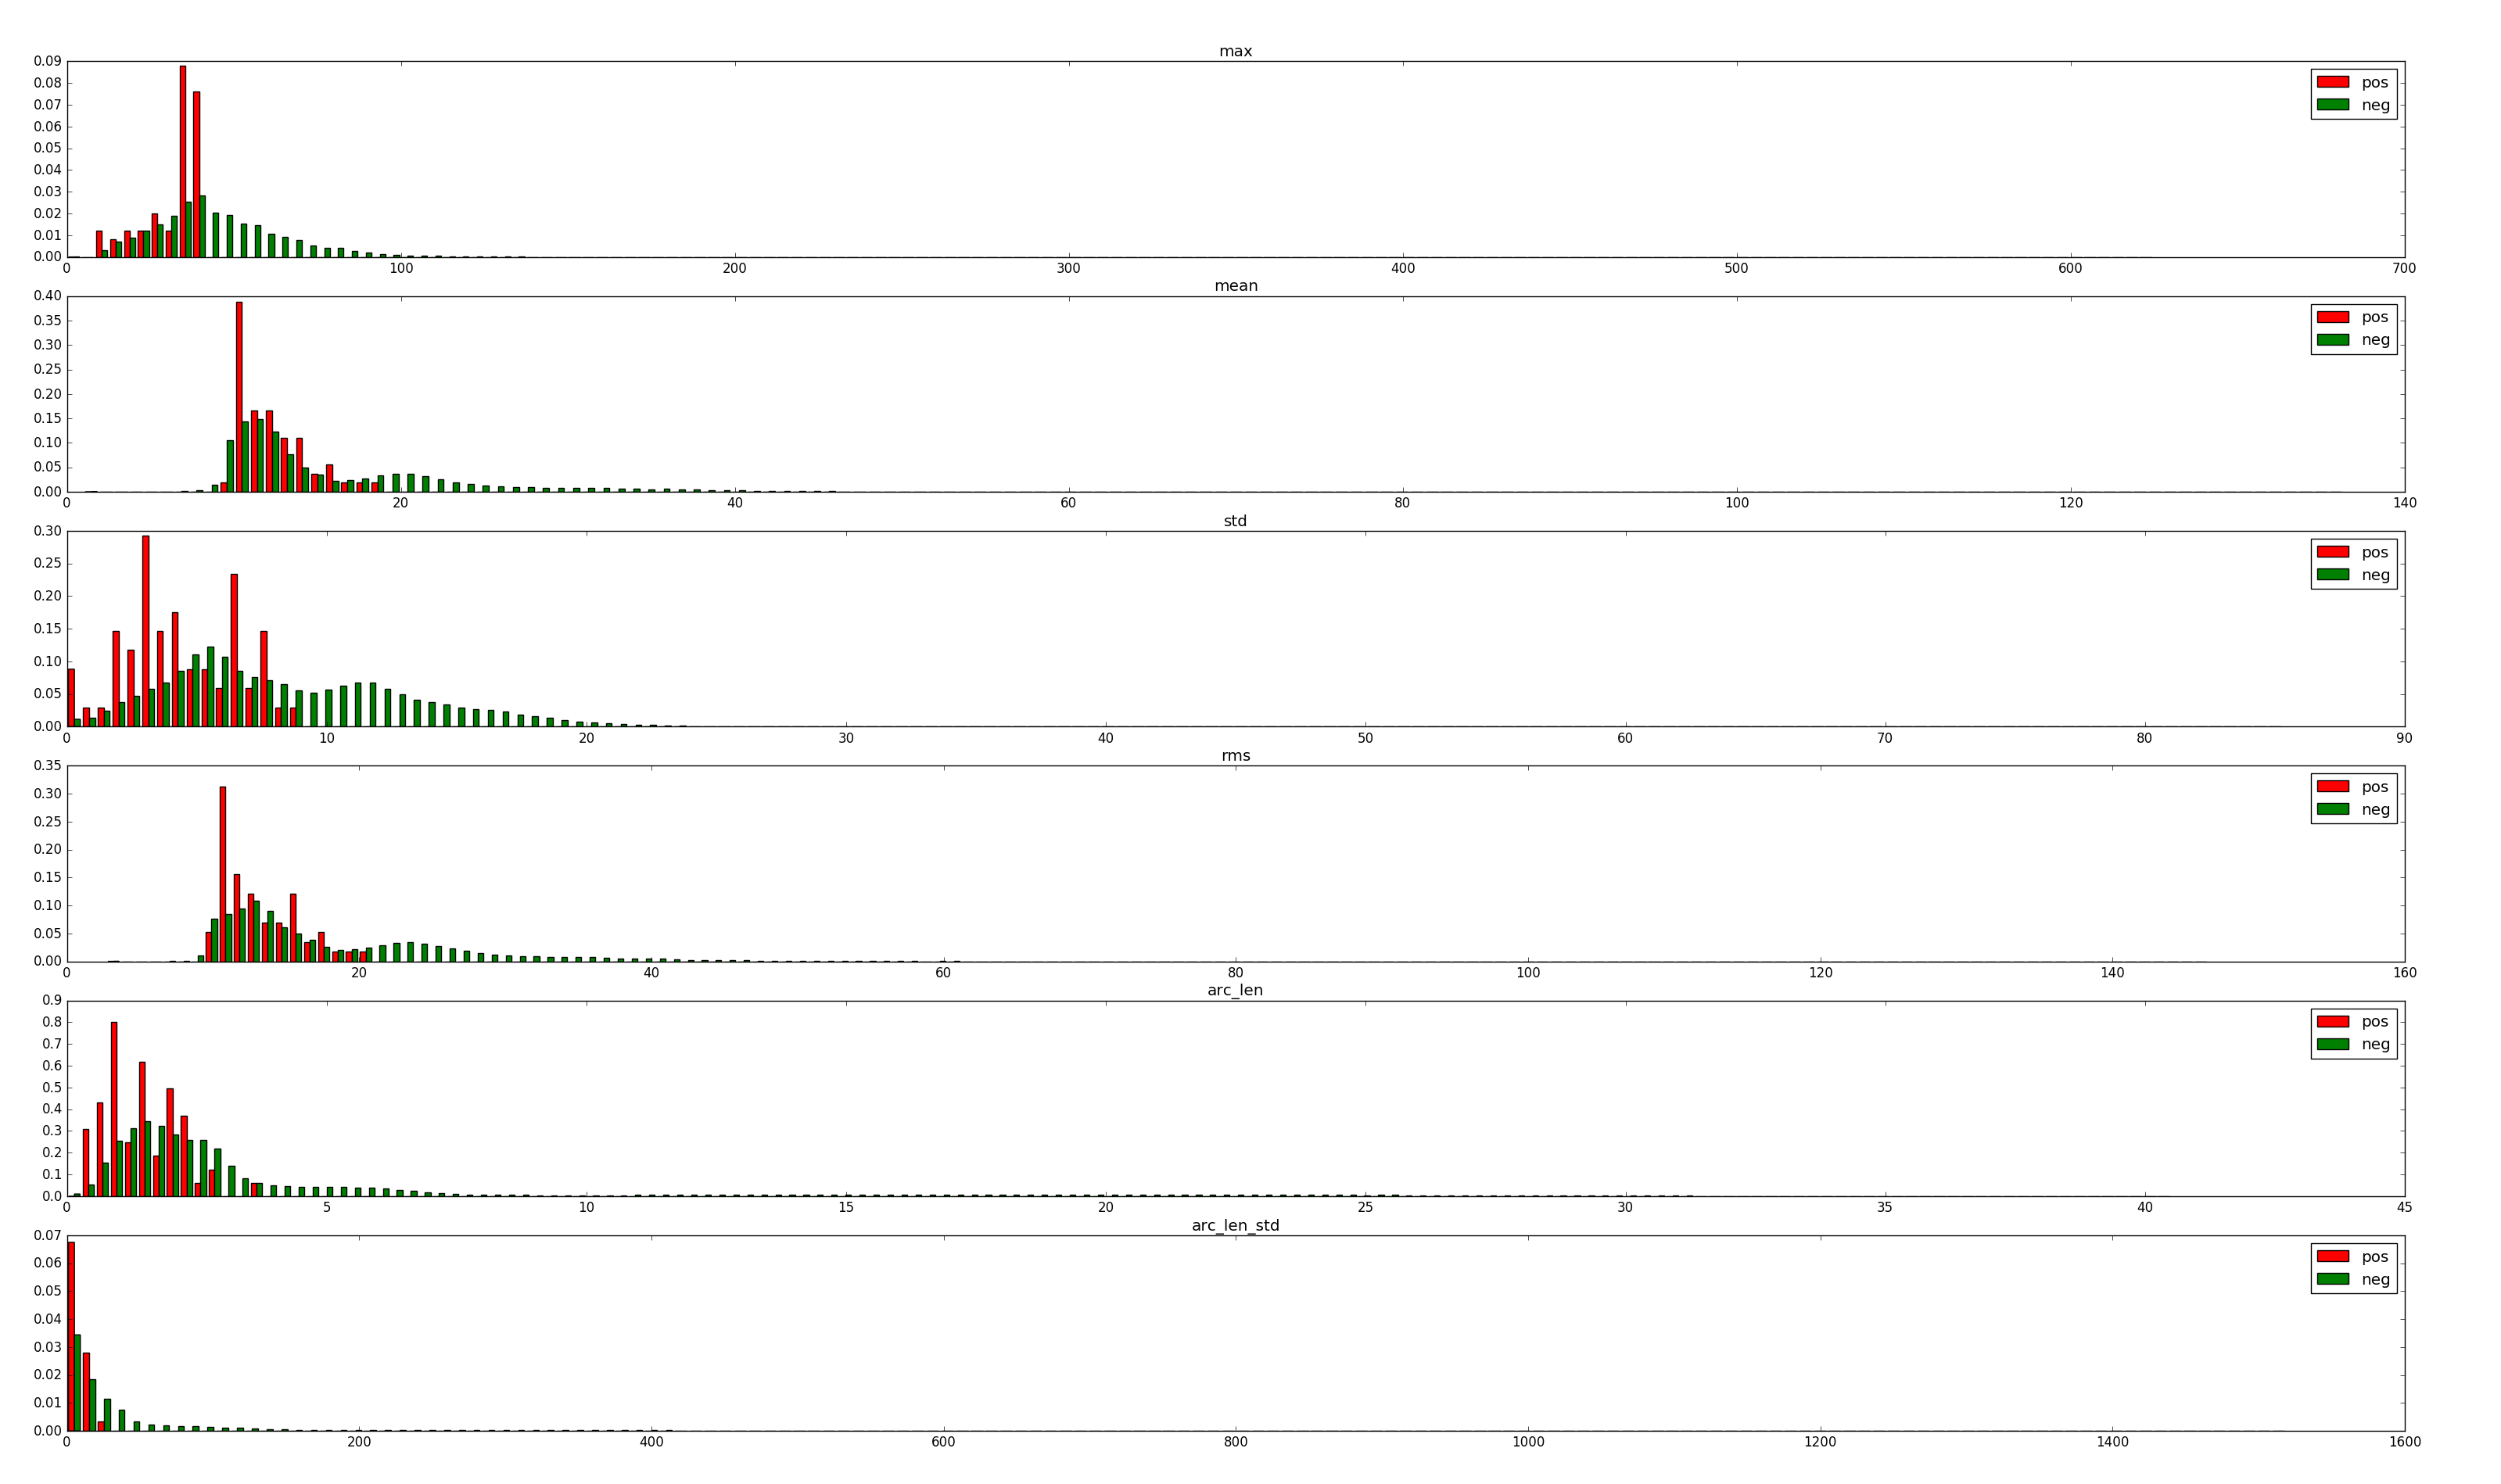
\includegraphics[width=\textwidth]{hist_features_before_win_size_1_2.png}
\caption{Histogram for each of the 6 features for the 1-second window before the~$40 m/s^2$ spike.  The features are listed in the order presented in Section~\ref{s:features}, e.g., the top histogram is for the maximum.  Red bars indicate thefts, and green bars indicate non-theft windows.}
\label{fig:beforehist}
\end{minipage}
\hfill
\begin{minipage}[t]{0.4\textwidth}
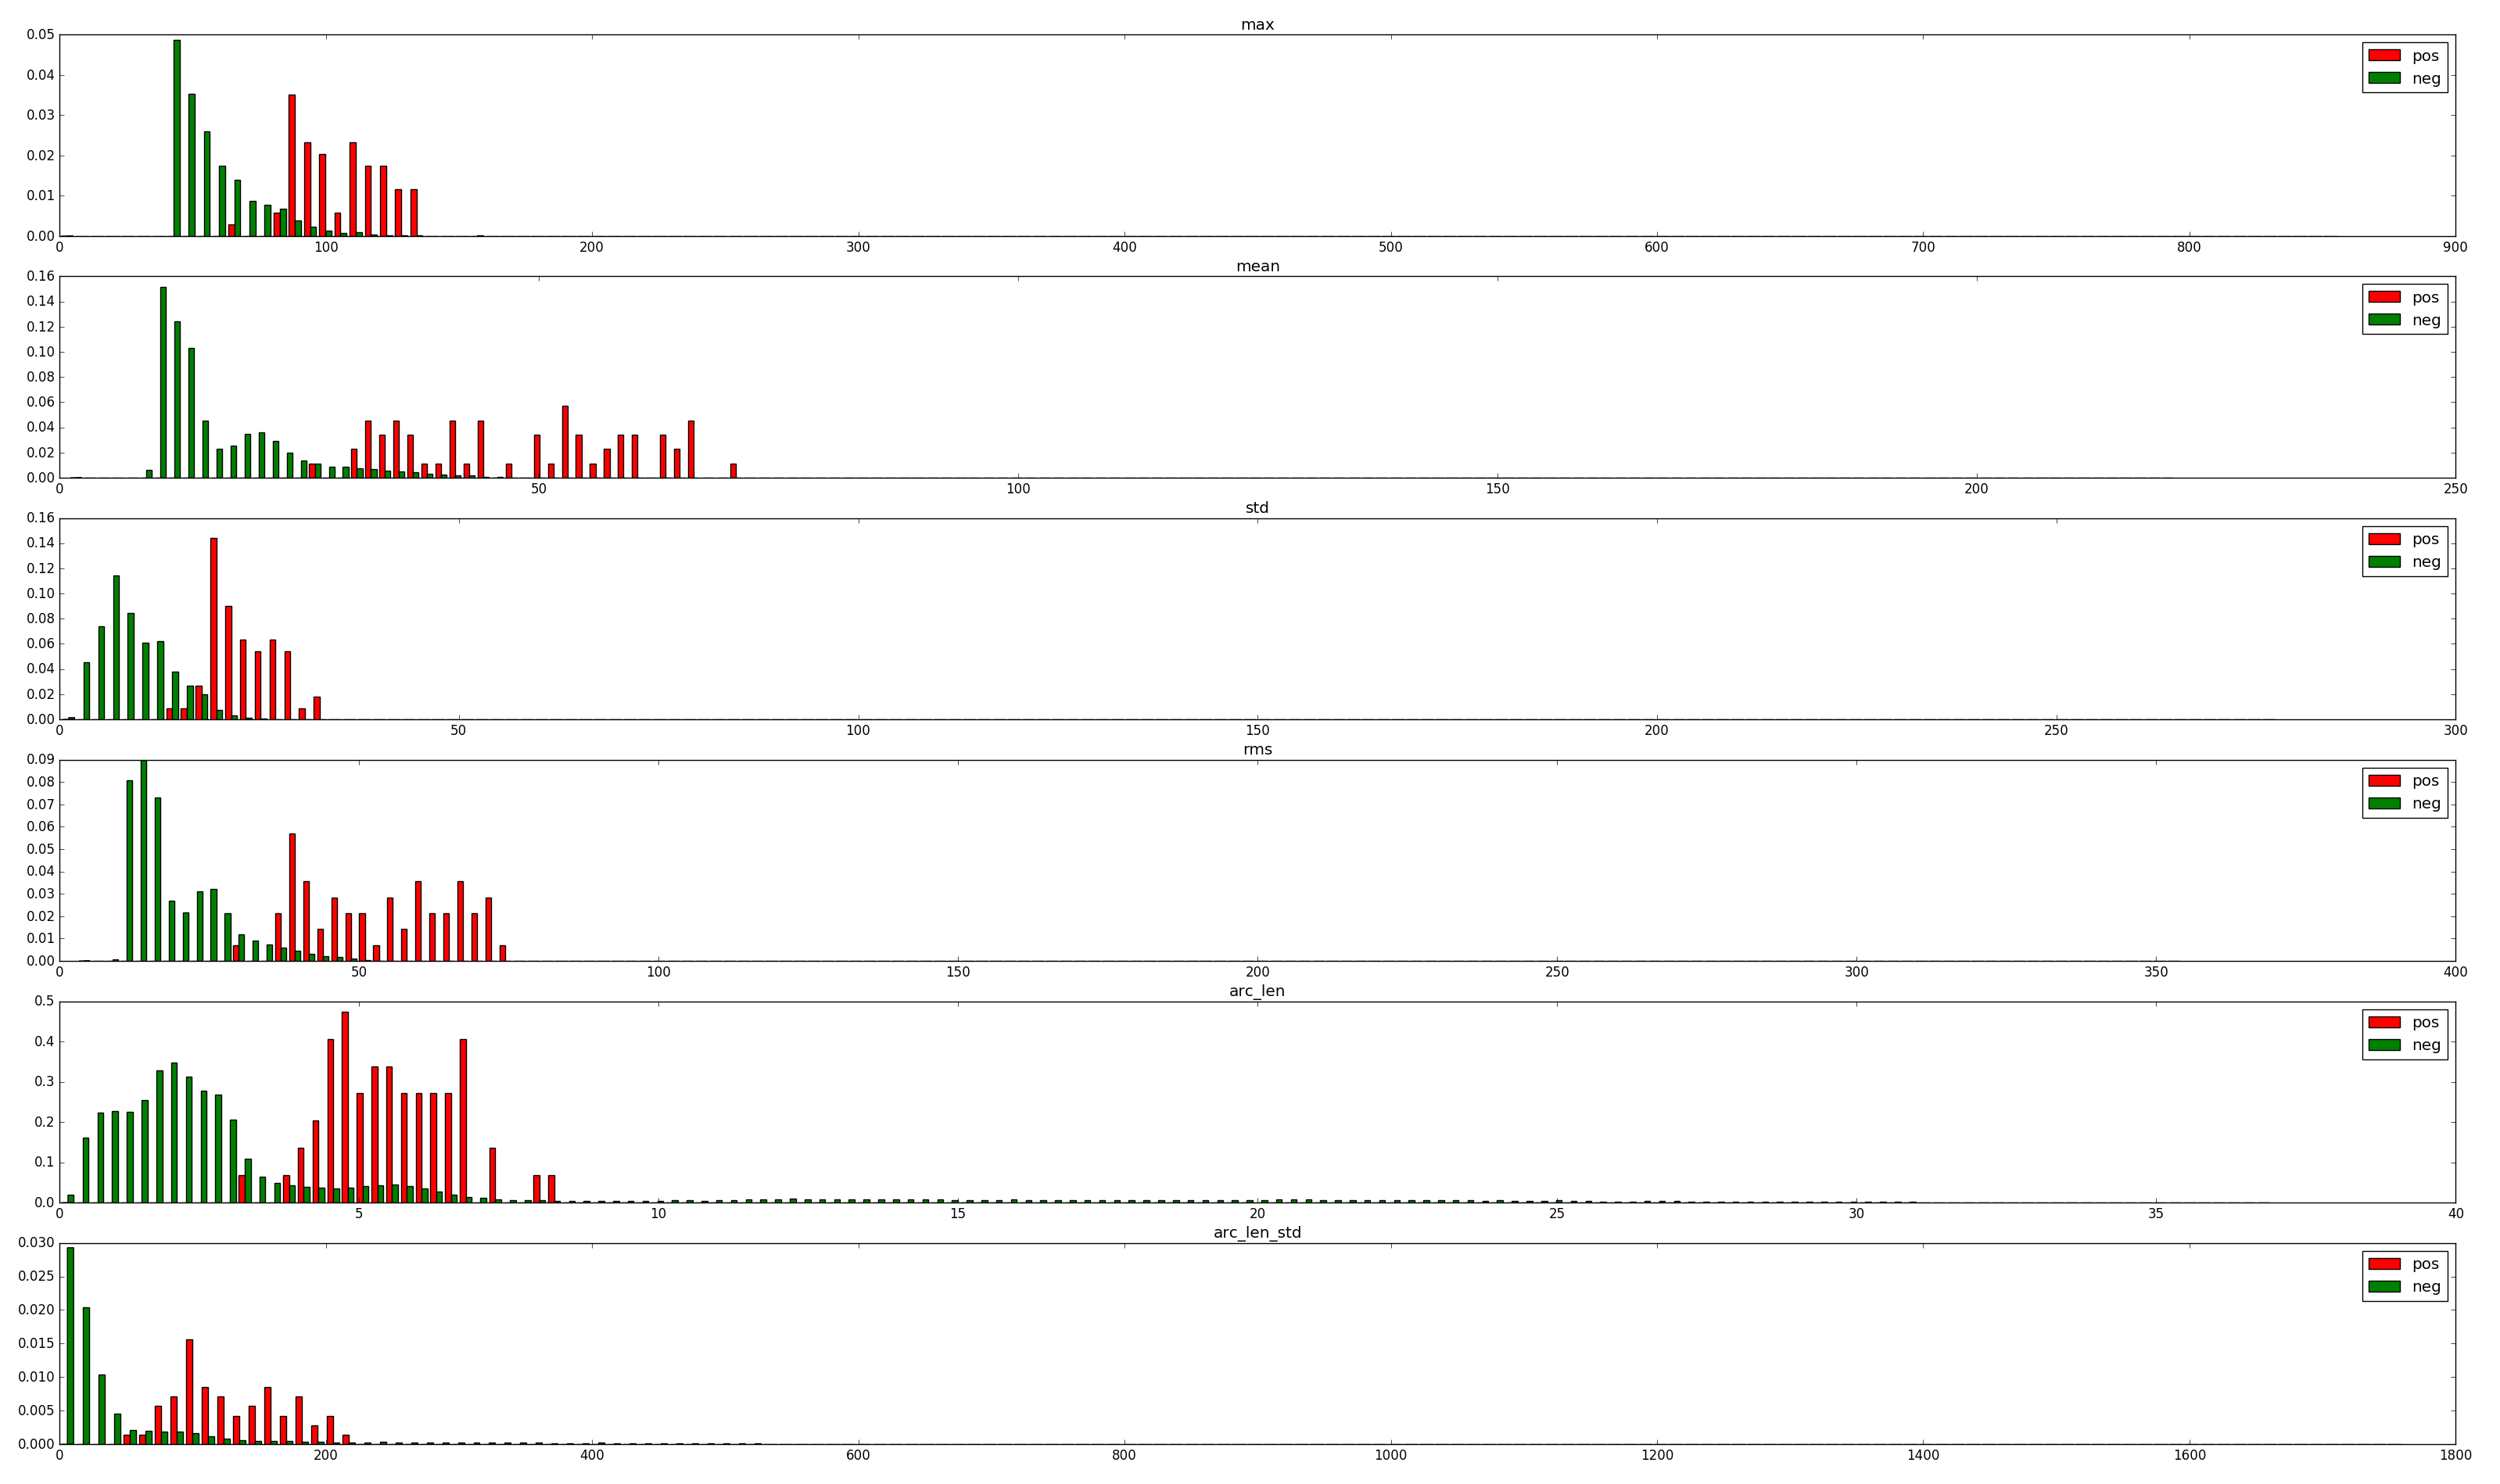
\includegraphics[width=\textwidth]{hist_features_after_win_size_1_2.png}
\caption{Histogram of feature values in the 2-second window after the~$40 m/s^2$ spike.}
\label{fig:afterhist}
\end{minipage}
\end{figure*}

% \begin{figure*}[t]
% \begin{center}
% 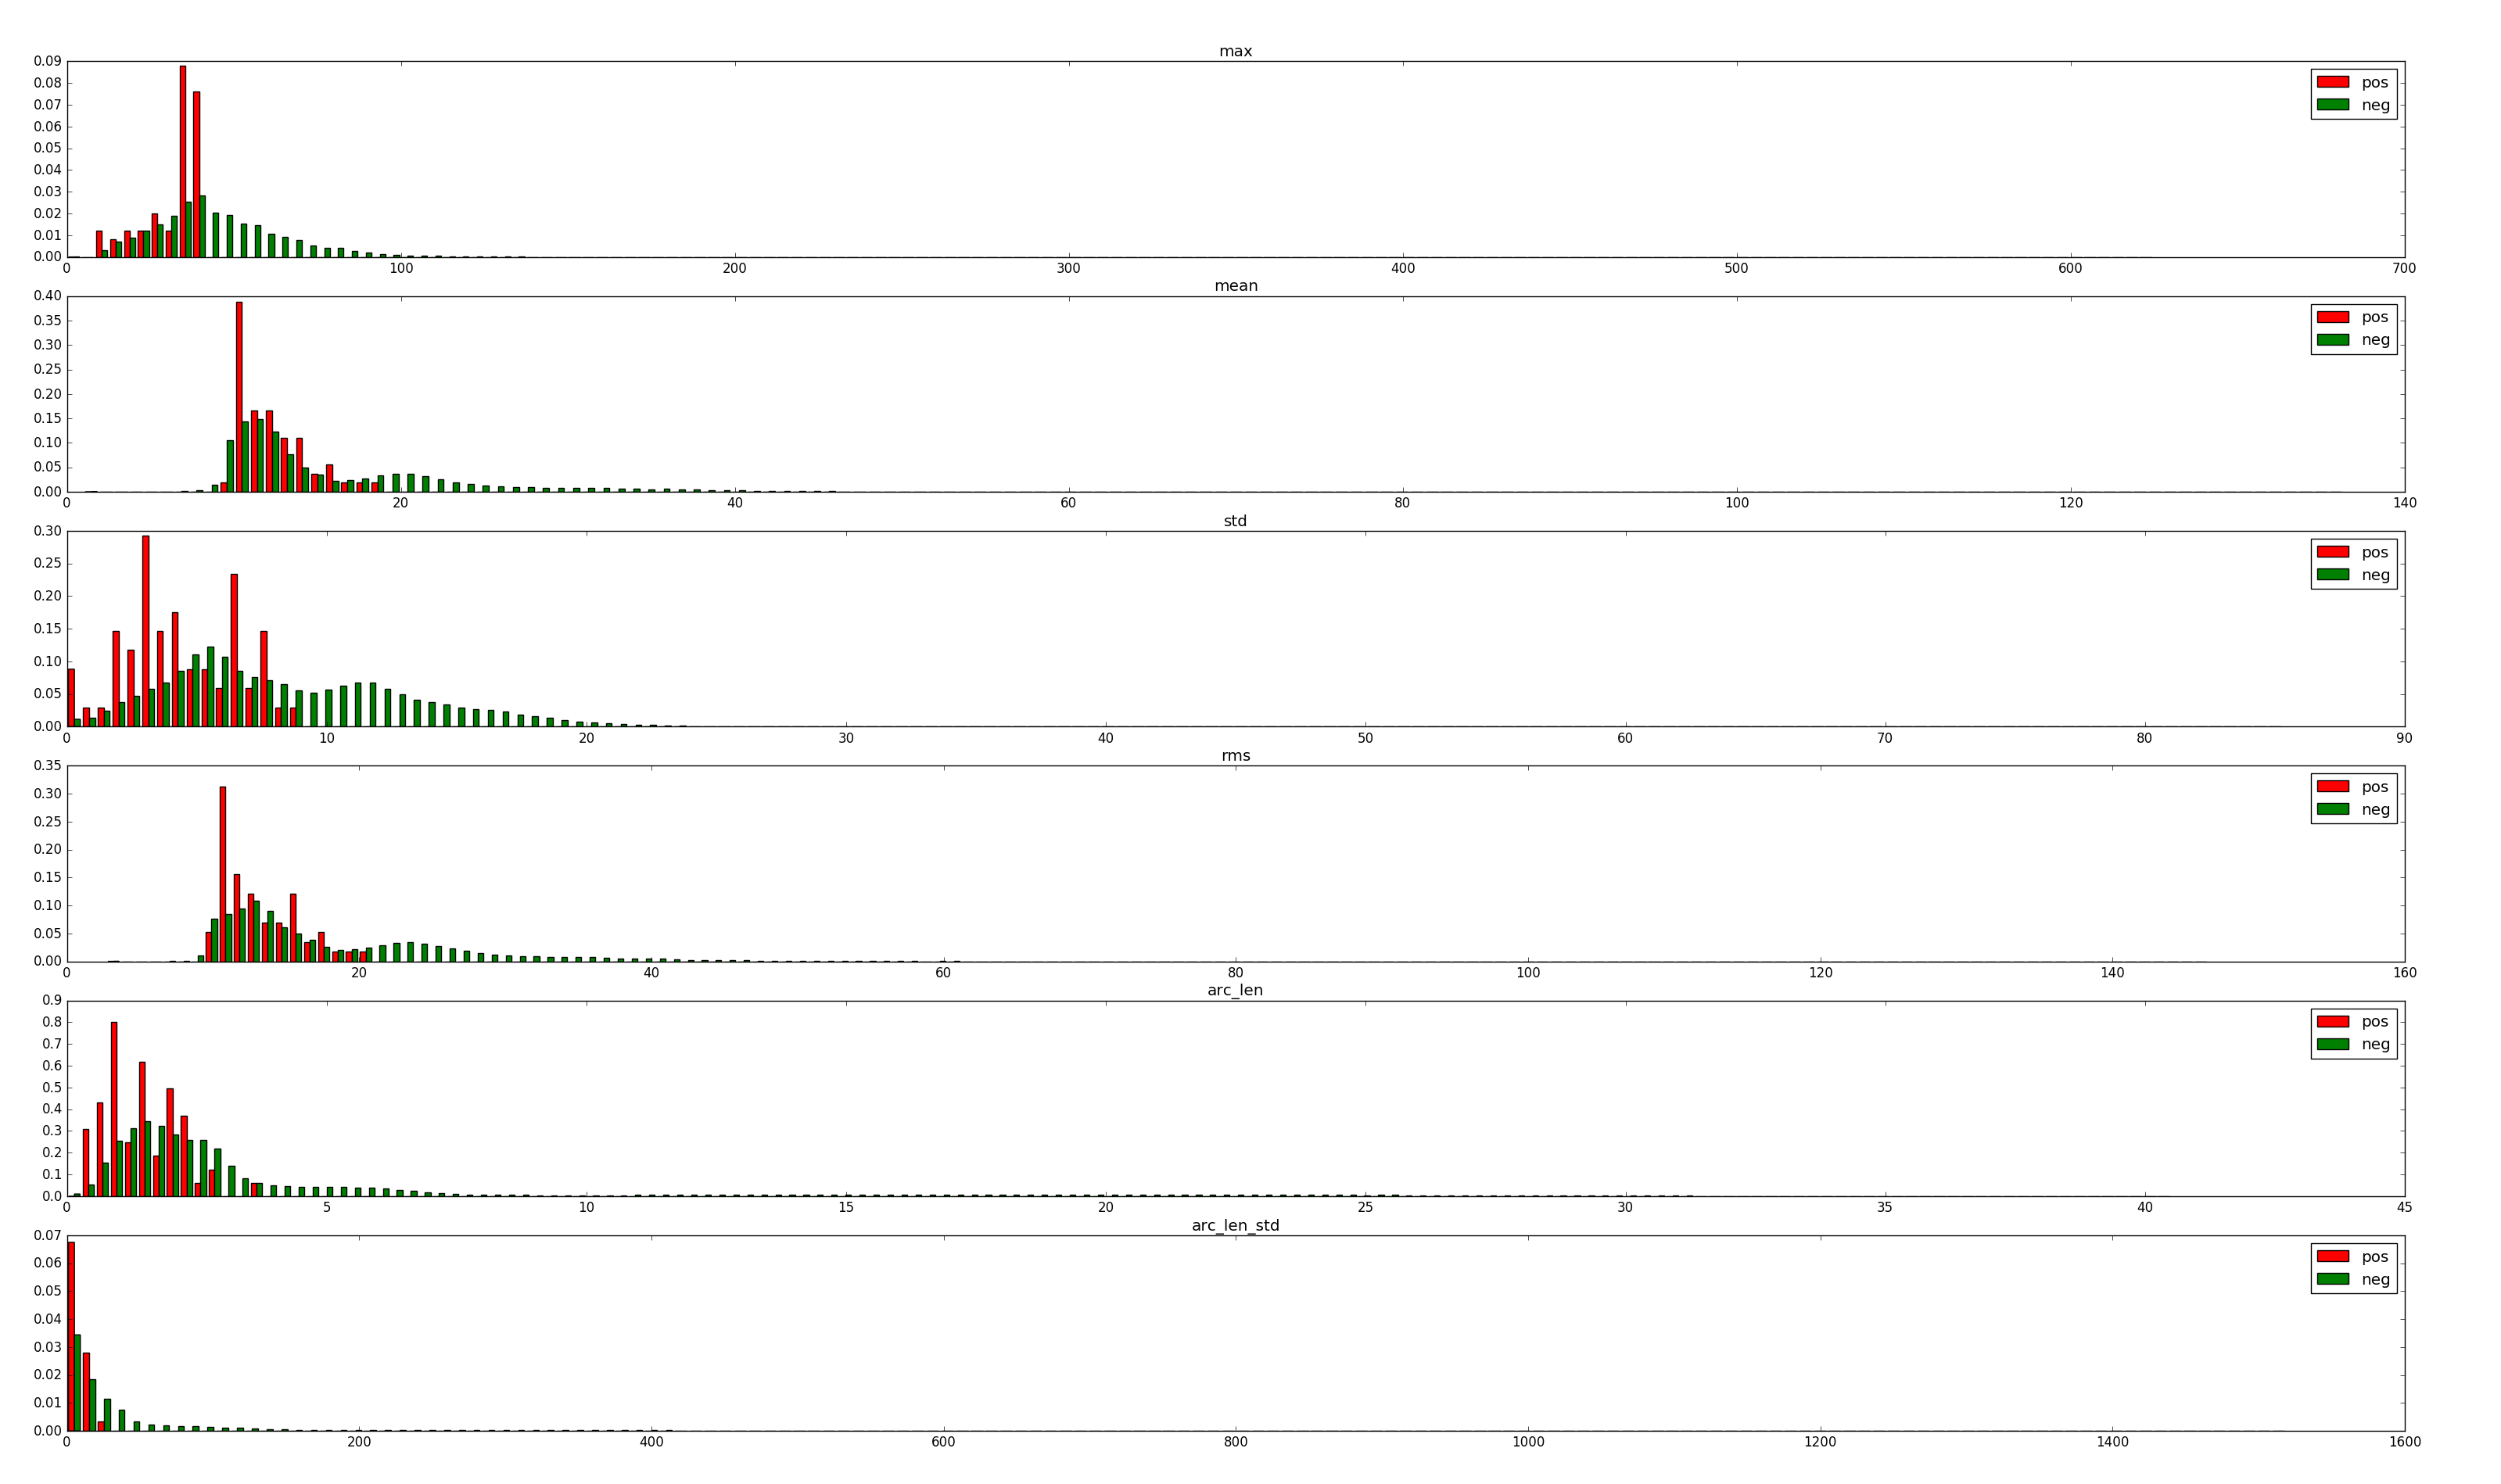
\includegraphics[width=\textwidth]{hist_features_before_win_size_1_2.png}
% \end{center}
% \caption{Histogram for each of the 6 features for the 1-second window before the~$40 m/s^2$ spike.  The features are listed in the order presented in Section~\ref{s:features}, e.g., the top histogram is for the maximum.  Red bars indicate thefts, and green bars indicate non-theft windows.}
% \label{fig:beforehist}
% \end{figure*}

% \begin{figure*}[t]
% \begin{center}
% 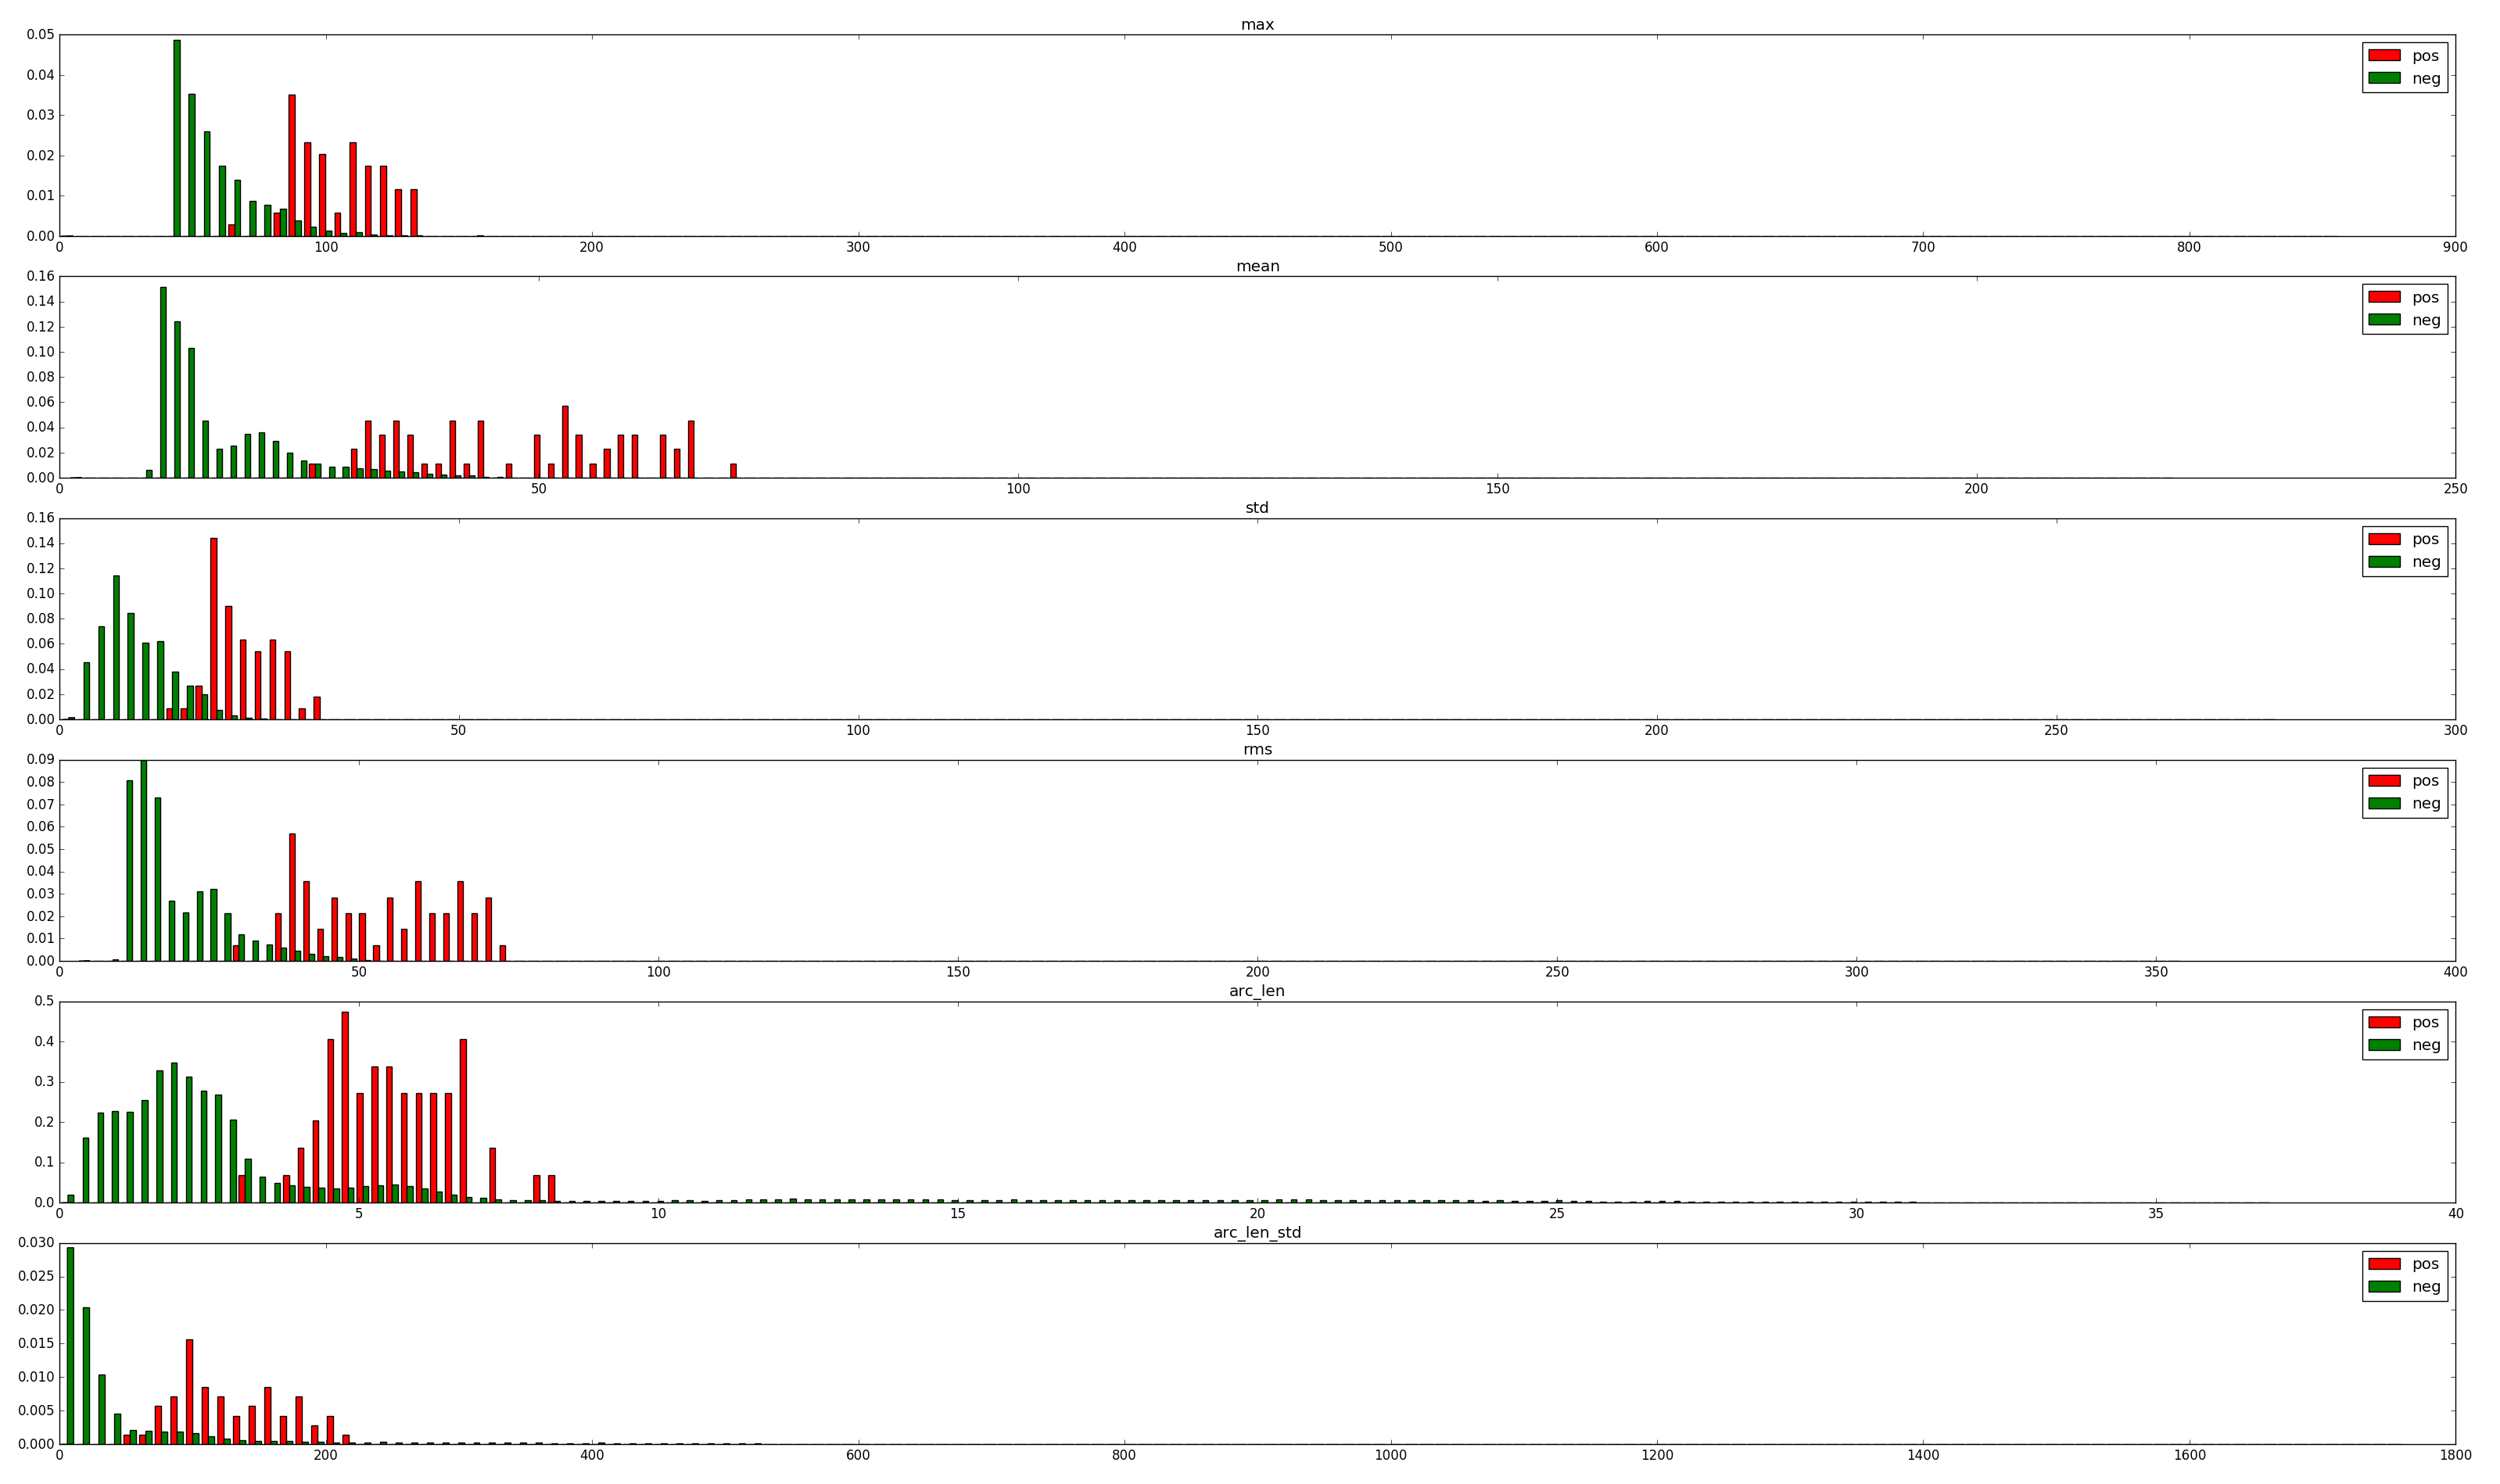
\includegraphics[width=\textwidth]{hist_features_after_win_size_1_2.png}
% \end{center}
% \caption{Histogram of feature values in the 2-second window after the~$40 m/s^2$ spike.}
% \label{fig:afterhist}
% \end{figure*}

To compare the performance of random forests and logistic regression, we finetune the class weights for the logistic regression classifier to lower its true positive rate until it is approximately the same as random forests classifier, then we compare the number of false positive instances of the two classifiers.
We find that logistic regression has 34 false positive instances at a 42\% true positive rate (25 true positive instances),
while random forests has 33 false positive instances at a 47\% true positive rate (28 true positive instances).
Thus the performance of the two classifiers seems comparable in this regime.
The advantage of logistic regression is that we found adjusting class weights was more effective at controlling the false-positive/false-negative tradeoff for the logistic regression classifier.
The Receiver Operating Characteristic (ROC) curves for the logistic regression and random forests classifiers are shown in Figure~\ref{fig:roc}.

\begin{figure}[t]
\begin{center}
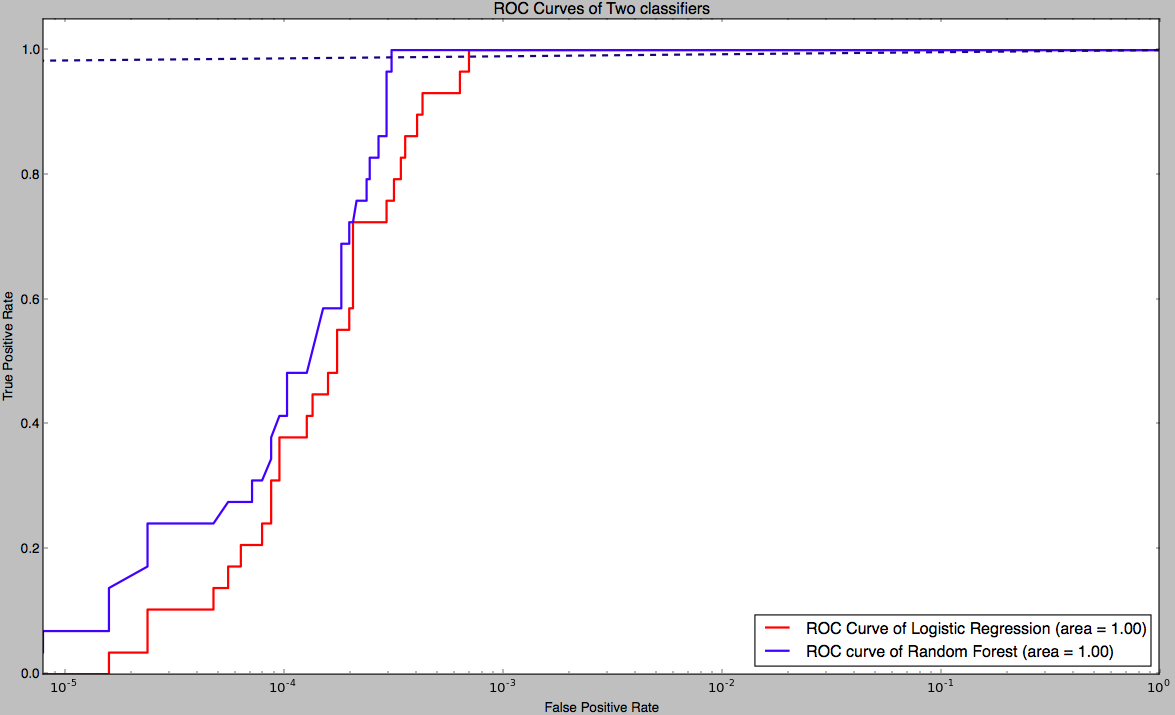
\includegraphics[width=1.0\columnwidth]{roc_curves_log_line.png}
\end{center}
\caption{ROC curves of logistic regression and random forests. The x-axis is in logarithmic scale.}
\label{fig:roc}
\end{figure}


